% Statistical Journal of the IAOS (SAGE) -- sagej class, SageV (Vancouver) references
\documentclass[Afour, times]{sagej}

\usepackage{multirow}
\usepackage{graphicx}
\usepackage{subcaption}
\usepackage[hyphens]{url}
\usepackage{amsmath,amssymb}
\usepackage{booktabs}
\usepackage{xcolor}

\geometry{a4paper, margin=1in}

\usepackage[colorlinks,bookmarksopen,bookmarksnumbered,citecolor=red,urlcolor=red]{hyperref}

\newcommand{\m}{$-$}
\newcommand{\todo}[1]{\textcolor{red}{[TODO: #1]}}
\newcommand{\SACA}{y^{\mathrm{SCA}}}
\newcommand{\DMR}{\mathrm{DMR}}

\def\volumeyear{2026}

\begin{document}
\setcounter{secnumdepth}{3}

\runninghead{Piovani}

\title{Building calendars for daily seasonal adjustment: lessons from electronic invoicing and electricity demand}

\author{Alessandro Piovani\affilnum{1}}

\affiliation{\affilnum{1}ISTAT, Directorate for Methodology and Statistical Process Design}

\corrauth{Alessandro Piovani, ISTAT, Directorate for Methodology and Statistical Process Design, Via Cesare Balbo 16, 00184 Rome}

\email{alessandro.piovani@istat.it}

\begin{abstract}
Daily administrative and transactional data are increasingly used as timely proxies for monthly indicators, but their seasonal adjustment needs a far richer calendar: special days that a monthly total averages out are visible, and large, in a daily series. We build calendars for two Italian daily series, the taxable amount of electronic invoices (2019--2025) and national electricity demand (2012--2025). Rather than the coefficients, we judge the adjusted series through a Day-to-Month Ratio (DMR), the ratio of each day to the median of its month, summarised by groups of days chosen according to the mechanism of each calendar effect. The same process leads to two very different calendars: an administrative calendar for e-invoicing, with month-end and deadline effects that depend on the day of the week, and a production calendar for electricity, with bridges, semi-closure days and holiday effects that drift over time. The final calendars bring almost all day groups within a $\pm5\%$ tolerance and make the most recent estimates more stable, with revisions on special days lower by about two thirds for electricity and by almost 90\% on holidays for e-invoicing, while standard diagnostics on rolling autocorrelations barely distinguish the calendars. We derive practical lessons for building daily calendars.
\end{abstract}

\keywords{Daily time series, seasonal adjustment, calendar effects, high-frequency data, revisions, JDemetra+}

\maketitle

% =============================================================================
\section{Introduction}
\label{sec:intro}

Daily administrative and transactional data are increasingly used by statistical offices and central banks as timely proxies for official monthly indicators. Their value lies in timeliness: a daily series that is seasonally and calendar adjusted makes partial months comparable, and can therefore be used to track a month before it closes. Seasonal adjustment of daily data, however, poses specific challenges: several periodicities that may be non-integer (weekly, monthly, annual), long series with structural changes, and a large number of calendar effects \cite{ollech2021,webel2022,webelsmyk2023,ollech2023}.

This paper focuses on the last of these challenges. On a daily basis, modelling the calendar is a central part of the methodological strategy, because daily data expose every special day that monthly or quarterly aggregation smooths out. In the two series we study, the last day of a month is worth almost nine ordinary weekdays of electronic invoicing, and a national holiday falling on a weekday removes about 150 thousand MWh from daily electricity demand, roughly a fifth of a normal day. Effects of this size cannot be left to the seasonal components, and a calendar that is only approximately right leaves residual patterns that are large on exactly the days that users look at: month ends, holidays and the days around them.

Calendar effects in monthly and quarterly data are well documented, and the standard tools are regressors for trading days, moving holidays and leap years estimated within a RegARIMA model \cite{bellhillmer1983,findley1998,essguidelines2015}. At daily frequency, the national holidays are only the starting point: their effect depends on the day of the week on which they fall, the days around them may also be affected, and many relevant days are not holidays at all, such as payment deadlines, month ends or plant closures. Methods for daily seasonal adjustment are now available \cite{ollech2021,proietti2023,webelsmyk2023}, but little guidance exists on how to build and validate the calendar for a specific series.

We address this question with two Italian daily series that differ in nature: the taxable amount of electronic invoices, related to business turnover, and national electricity demand, related to industrial production. Both are adjusted with the JDemetra+~3 R packages \cite{webelsmyk2023,rjdverse}. Our contributions are four. First, we propose a diagnostic based on the adjusted series rather than on the estimated coefficients, the Day-to-Month Ratio (DMR), summarised by groups of days that follow the mechanism behind each calendar effect. Second, we describe an iterative building process in which each regressor is motivated by a hypothesis, checked with a dedicated DMR chart and retained only if it improves the adjusted series. Third, we show that the same process leads to two very different calendars, an \emph{administrative} calendar for e-invoicing and a \emph{production} calendar for electricity, and derive lessons for good practice. Finally, we show with a revision analysis that, for both series, the final calendar also stabilises the most recent estimates, above all on special days.

Section~\ref{sec:data} describes the data and Section~\ref{sec:methods} the models, the DMR and the building process. Sections~\ref{sec:einv} and~\ref{sec:el} present the two calendars, and Section~\ref{sec:rev} analyses the revisions of both series. Section~\ref{sec:kde} compares the DMR with a standard diagnostic based on rolling autocorrelations. Section~\ref{sec:discussion} discusses lessons and limitations, and Section~\ref{sec:conclusions} concludes.

% =============================================================================
\section{Data}
\label{sec:data}

\textit{Electronic invoicing.} In Italy, invoices between businesses have been issued electronically through a central exchange system since 2019. We use the daily taxable amount of electronic invoices from 1 January 2019 to 31 December 2025 (2,557 days), a candidate proxy for business turnover \todo{add data source, coverage and units}. The series has a very strong intra-month pattern (Figure~\ref{fig:raw}a): businesses concentrate invoicing at the end of the month, and administrative rules create further peaks, for instance on the 15th, the deadline for deferred invoices relating to the previous month's deliveries.

\textit{Electricity demand.} Daily national electricity demand from 1 January 2012 to 31 December 2025 (5,114 days), measured in MWh, is a high-frequency proxy for industrial production \todo{add data source (transmission system operator)}. The series has a strong weekly pattern, a double annual peak (winter heating and summer cooling) and deep troughs on holidays, in mid-August and over Christmas (Figure~\ref{fig:raw}b).

\begin{figure*}[t]
\centering
\begin{subfigure}{0.9\textwidth}
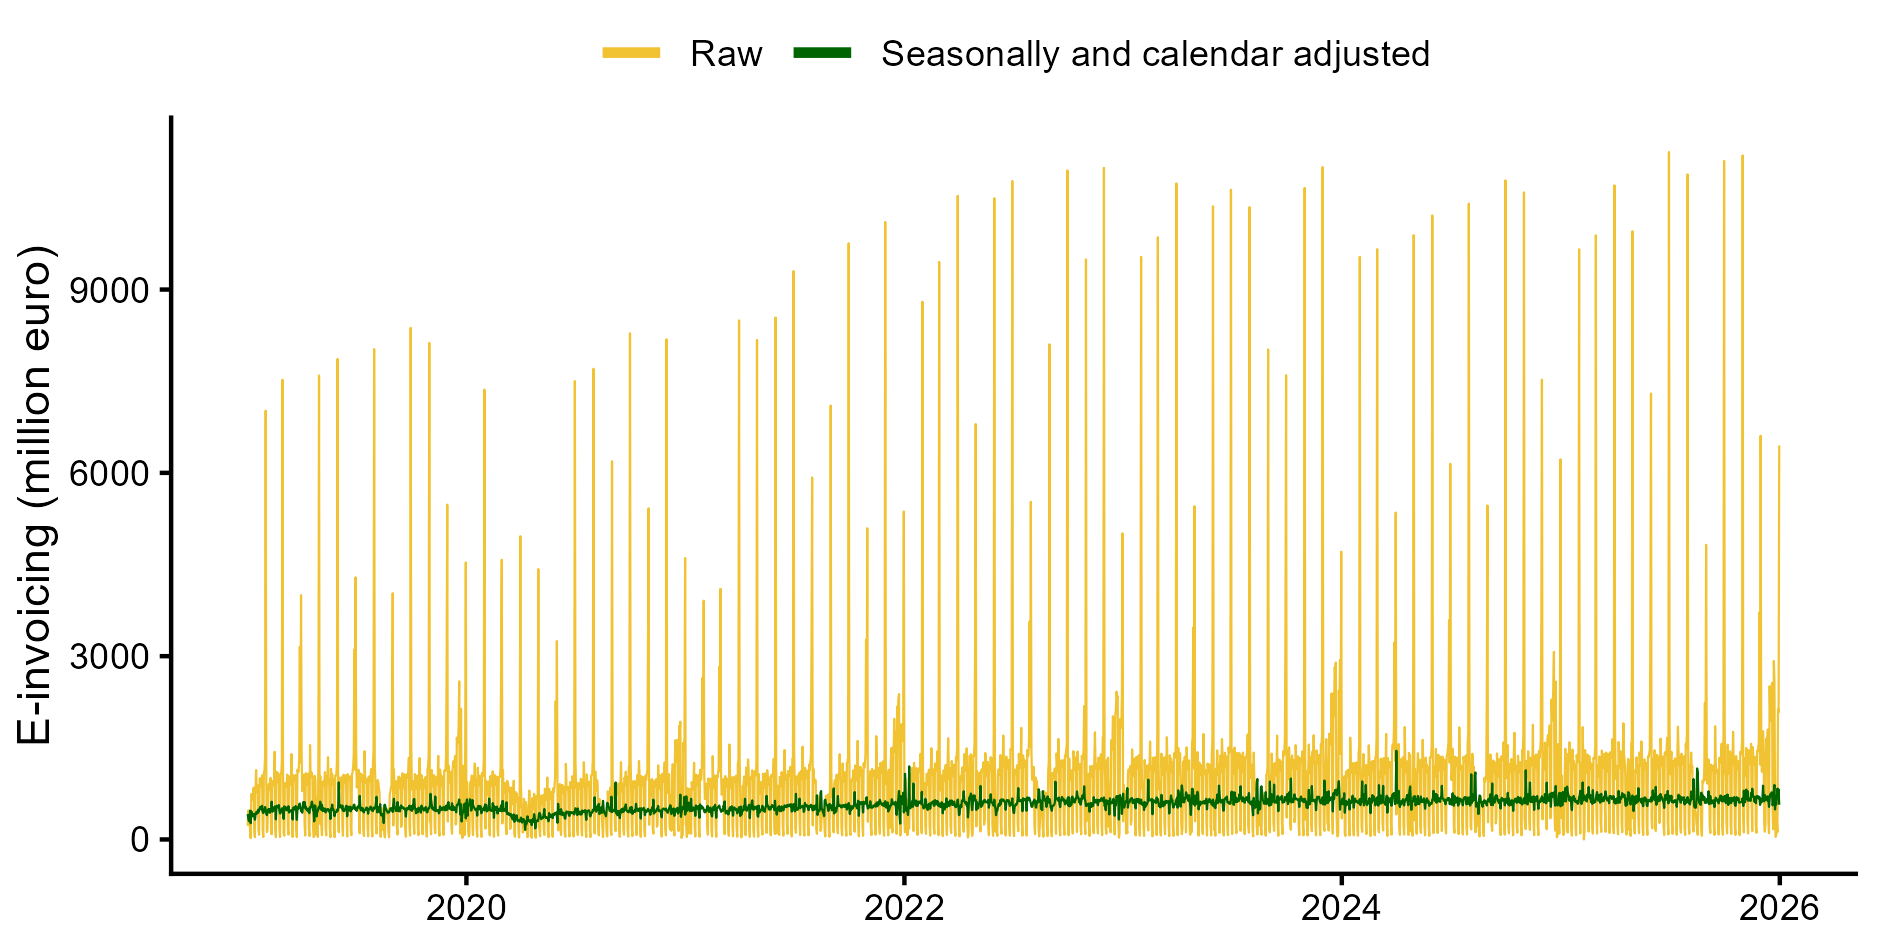
\includegraphics[width=\linewidth]{figures/raw_sa_einvoicing.png}
\caption{Electronic invoicing (multiplicative model)}
\end{subfigure}

\vspace{6pt}
\begin{subfigure}{0.9\textwidth}
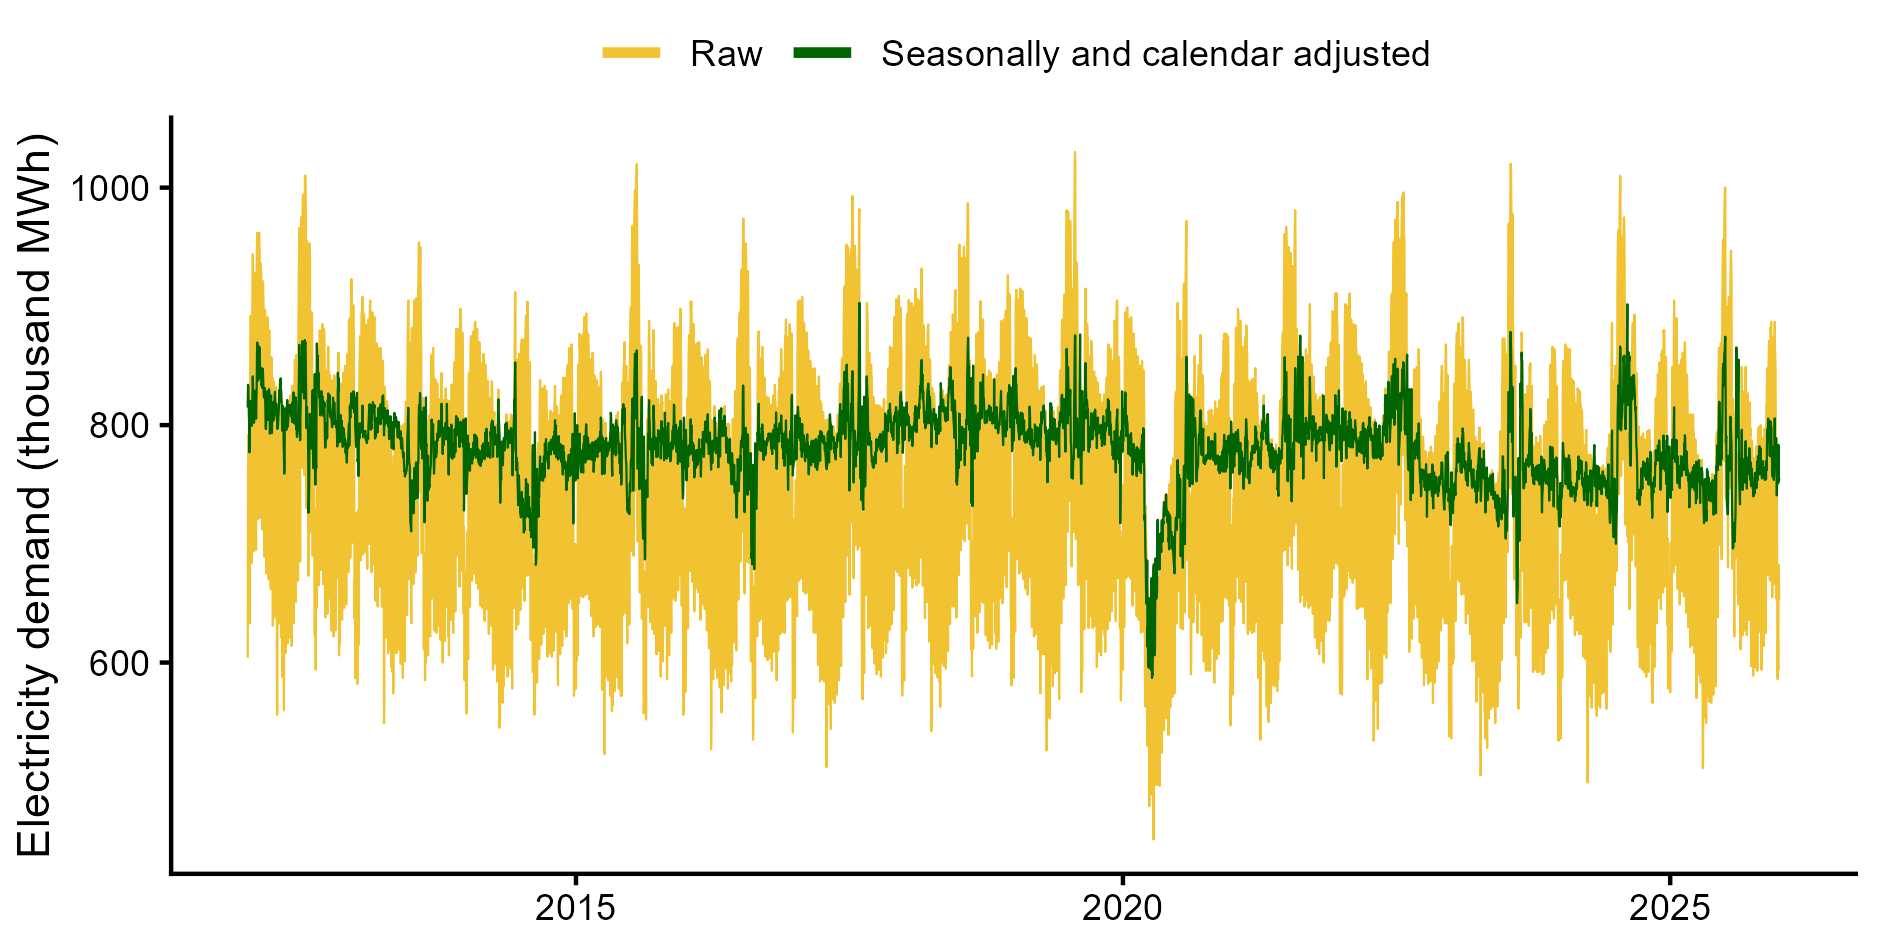
\includegraphics[width=\linewidth]{figures/raw_sa_electricity.png}
\caption{Electricity demand (additive model)}
\end{subfigure}
\caption{Raw series and seasonally and calendar adjusted series obtained with the final calendars.}
\label{fig:raw}
\end{figure*}

% =============================================================================
\section{Methods}
\label{sec:methods}

\subsection{Pre-treatment and decomposition}
\label{subsec:model}

Both series are adjusted with the R packages \texttt{rjd3toolkit}, \texttt{rjd3highfreq} and \texttt{rjd3sts} of JDemetra+~3 \cite{rjdverse}. A test on the corrected Akaike criterion (AICc) of an extended airline model with periods 7 and 365.2425 selects a multiplicative (log) model for e-invoicing and an additive model for electricity.

The pre-treatment estimates an extended (fractional) airline model with periods 7 and 365.2425 \cite{webelsmyk2023}, with automatic detection of additive outliers (AO), switch outliers (WO) and level shifts (LS) above a critical value of 6. The linearised series is then decomposed with a sequential ARIMA-model-based (AMB) approach: the weekly component is extracted first, and the annual component is then extracted from the weekly adjusted series. Level shifts are added back to the adjusted series, since they represent changes in level rather than calendar or seasonal effects. The output of interest is the seasonally and calendar adjusted series, denoted $\SACA_t$ (SCA); the seasonally adjusted series is obtained by adding the calendar component back.

Calendar effects are handled in two ways. With \emph{fixed coefficients}, used for e-invoicing, the calendar regressors enter the pre-treatment model and are estimated jointly with the ARIMA parameters and the outliers. With \emph{time-varying coefficients}, used for electricity, the calendar component is estimated in a preliminary state-space model and removed before the pre-treatment (Section~\ref{subsec:tv}).

\subsection{Time-varying calendar effects}
\label{subsec:tv}

Let $z_t$ be the observed series (in logs for a multiplicative model) and $X_{k,t}$, $k=1,\dots,K$, binary calendar regressors. The model is a regression with time-varying coefficients and weekly airline errors:
\begin{align}
z_t &= \sum_{k=1}^{K} \beta_{k,t}\, X_{k,t} + u_t, \label{eq:obs}\\
(1-B)(1-B^7)\, u_t &= (1-\theta B)(1-\Theta B^7)\, \nu_t, \label{eq:airline}\\
\beta_{k,t} &= \beta_{k,t-1} + \xi_{k,t}, \label{eq:rw}
\end{align}
where $B$ is the backshift operator, $\nu_t \sim N(0,\sigma^2_\nu)$ and $\xi_{k,t} \sim N(0,\sigma^2_\xi)$, independent of $\nu_t$. The coefficients follow random walks with a common variance $\sigma^2_\xi$; with $\sigma^2_\xi = 0$ the model reduces to fixed coefficients, so the likelihood ratio between the two specifications measures the evidence for time variation. The model is cast in state-space form, with the coefficients in the state vector, and estimated by maximum likelihood with the Kalman filter; the smoothed coefficients give the calendar component
\begin{align}
H_t &= \sum_{k=1}^{K} \beta_{k,t}\, X_{k,t}, \label{eq:H}\\
z^{CA}_t &= z_t - H_t, \nonumber
\end{align}
and the calendar-adjusted series $z^{CA}_t$ goes through the pre-treatment, for outliers only, and the AMB decomposition \cite{durbinkoopman2012}. The weekly airline in~\eqref{eq:airline} captures the weekly pattern; the annual pattern is left to the subsequent decomposition. This two-step approach has a cost, discussed in Section~\ref{sec:discussion}: the calendar is estimated against a model with weekly seasonality only.

\subsection{The Day-to-Month Ratio}
\label{subsec:dmr}

Calendar regressors are usually assessed through the significance of their coefficients. A significant coefficient, however, does not guarantee that the adjusted series is free of calendar effects: a regressor can be significant and still leave a large residual pattern, for instance when one coefficient is forced to fit days with very different base levels. We therefore assess the calendar on the adjusted series. For each day $t$ we define
\begin{equation}
\DMR_t = \frac{\SACA_t}{\operatorname{median}\{\SACA_m : m \in M(t)\}}, \label{eq:dmr}
\end{equation}
where $M(t)$ is the set of days in the month of $t$. If the calendar is correctly specified, no group of days is systematically above or below its month, and the median DMR is close to 1 for any group of days. This does not require the adjusted series to be flat within each month: genuine short-term movements remain in $\DMR_t$, but they are not tied to particular days and cancel out in the group medians. For a group $g$ of days we compute the median $\widetilde{\DMR}_g = \operatorname{median}\{\DMR_t : t \in g\}$ over the whole sample; medians are robust to outliers and to unusual months. A group is considered adjusted when $\widetilde{\DMR}_g$ lies within $1 \pm 0.05$. A value above or below 1 indicates under- or over-correction, depending on the sign of the calendar effect. The DMR is computed in the same way for multiplicative and additive models.

The denominator is always the monthly median; what changes is the grouping of days, which must follow the mechanism of the effect under study:
\begin{itemize}
\item \emph{day of the week}, to check that the weekly pattern has been removed;
\item \emph{day of the month}, for effects tied to fixed dates (payment deadlines, day 1, day 15);
\item \emph{days to the end of the month}, for month-end effects: grouping by day of the month would mix months of different length, since the 29th is the last day of a leap February and the third-last day of a 31-day month;
\item \emph{distance from each holiday}, from three days before to three days after, split by the weekday on which the holiday falls, to reveal bridges;
\item \emph{special periods} (Christmas to Epiphany, mid-August, the Easter week), by date.
\end{itemize}
Each critical group is then split by type of day (Monday to Friday, Saturday, Sunday). A median close to 1 can hide opposite errors on different types of day, and a misspecified regressor typically produces exactly this pattern (Section~\ref{sec:einv}). Finally, the list of outliers is part of the diagnostic. Outliers and calendar effects must be kept apart: an outlier on a holiday or on a nearby day, such as a bridge, signals a misspecified calendar rather than an unusual event. The regressor may be missing, or present but wrong, in which case the outlier falls on the very day the calendar models and offsets its effect (Section~\ref{sec:einv}).

\subsection{The building process}
\label{subsec:process}

The calendar is built iteratively. (i) The raw series is explored to find the days with recurring anomalies and, for each of them, a possible cause: holidays, month ends, deadlines, closures. (ii) A minimal and motivated calendar is specified, starting from the national holidays. (iii) The adjusted series is diagnosed with the DMR charts; groups outside the tolerance suggest hypotheses, each of which is checked with a dedicated chart before a regressor is added. (iv) Regressors are added one at a time, or in homogeneous groups, and all charts are redrawn after each change, because a correction can move the problem to the neighbouring days. (v) Once the diagnostics are satisfactory, the calendar is simplified: non-significant regressors are dropped and regressors with similar coefficients are merged, and the charts are checked again. Time variation is tested on the complete calendar. The process stops when all groups are within the tolerance, to avoid chasing effects that concern a handful of days.

As a benchmark we use a \emph{basic calendar} that a practitioner might adopt as a first step: the twelve Italian national holidays (including Easter Sunday and Easter Monday), active on every day of the week, with fixed coefficients; for e-invoicing, dummies for the last day of the month and the two preceding days are added.

% =============================================================================
\section{Electronic invoicing: an administrative calendar}
\label{sec:einv}

\subsection{What the basic calendar leaves}

With the basic calendar, the e-invoicing SCA series shows a strong intra-month pattern. By day of the month, the median DMR is 1.13 on day 1, 1.27 on day 15 and 1.09 on day 20, and falls to 0.82 and 0.76 on days 30 and 31. By days to the end of the month, the last day and the day before are over-corrected (0.79 and 0.82), while the third to fifth days before the month end are under-corrected (1.06--1.11): the month-end dummy absorbs part of a ramp that starts several days earlier. The peak on day 15 has an administrative explanation, since deferred invoices must be issued by the 15th of the month following delivery; the peak on day 20 may reflect invoicing at ten-day intervals, an hypothesis we could not verify.

Holidays active on every day of the week produce a clear failure: holidays falling on weekdays have a median DMR of 0.6--0.7, holidays falling on Saturdays and Sundays about 3. A Christmas on a Sunday receives the effect of a Christmas on a weekday, which cuts invoicing to a few per cent of a normal day, and a day on which invoicing is already low is heavily over-corrected. In an earlier specification, 11 of the 13 outliers detected fell on weekend holidays, with coefficients that almost exactly cancelled the holiday effect.

\subsection{The key choice: one coefficient per type of day}

Splitting the DMR by type of day reveals the main misspecification (Figure~\ref{fig:einv_daytype}). The last day of the month has a median DMR of 0.73 on weekdays, 1.96 on Saturdays and 4.3 on Sundays: a single coefficient cannot fit all three. The reason is that each calendar effect is relative to a normal day of the same type. Firms date their invoices on the last day of the month even when it falls on a Sunday, and a normal Sunday has very few invoices; the month-end multiplier is therefore much larger on Sundays than on weekdays, and a common coefficient is a compromise that over-corrects weekdays and under-corrects weekends. The same pattern appears for the other special days: in an intermediate specification with one dummy per day, day 15 had a median DMR of 0.89 on weekdays and 2.12 on Sundays.

\begin{figure*}[t]
\centering
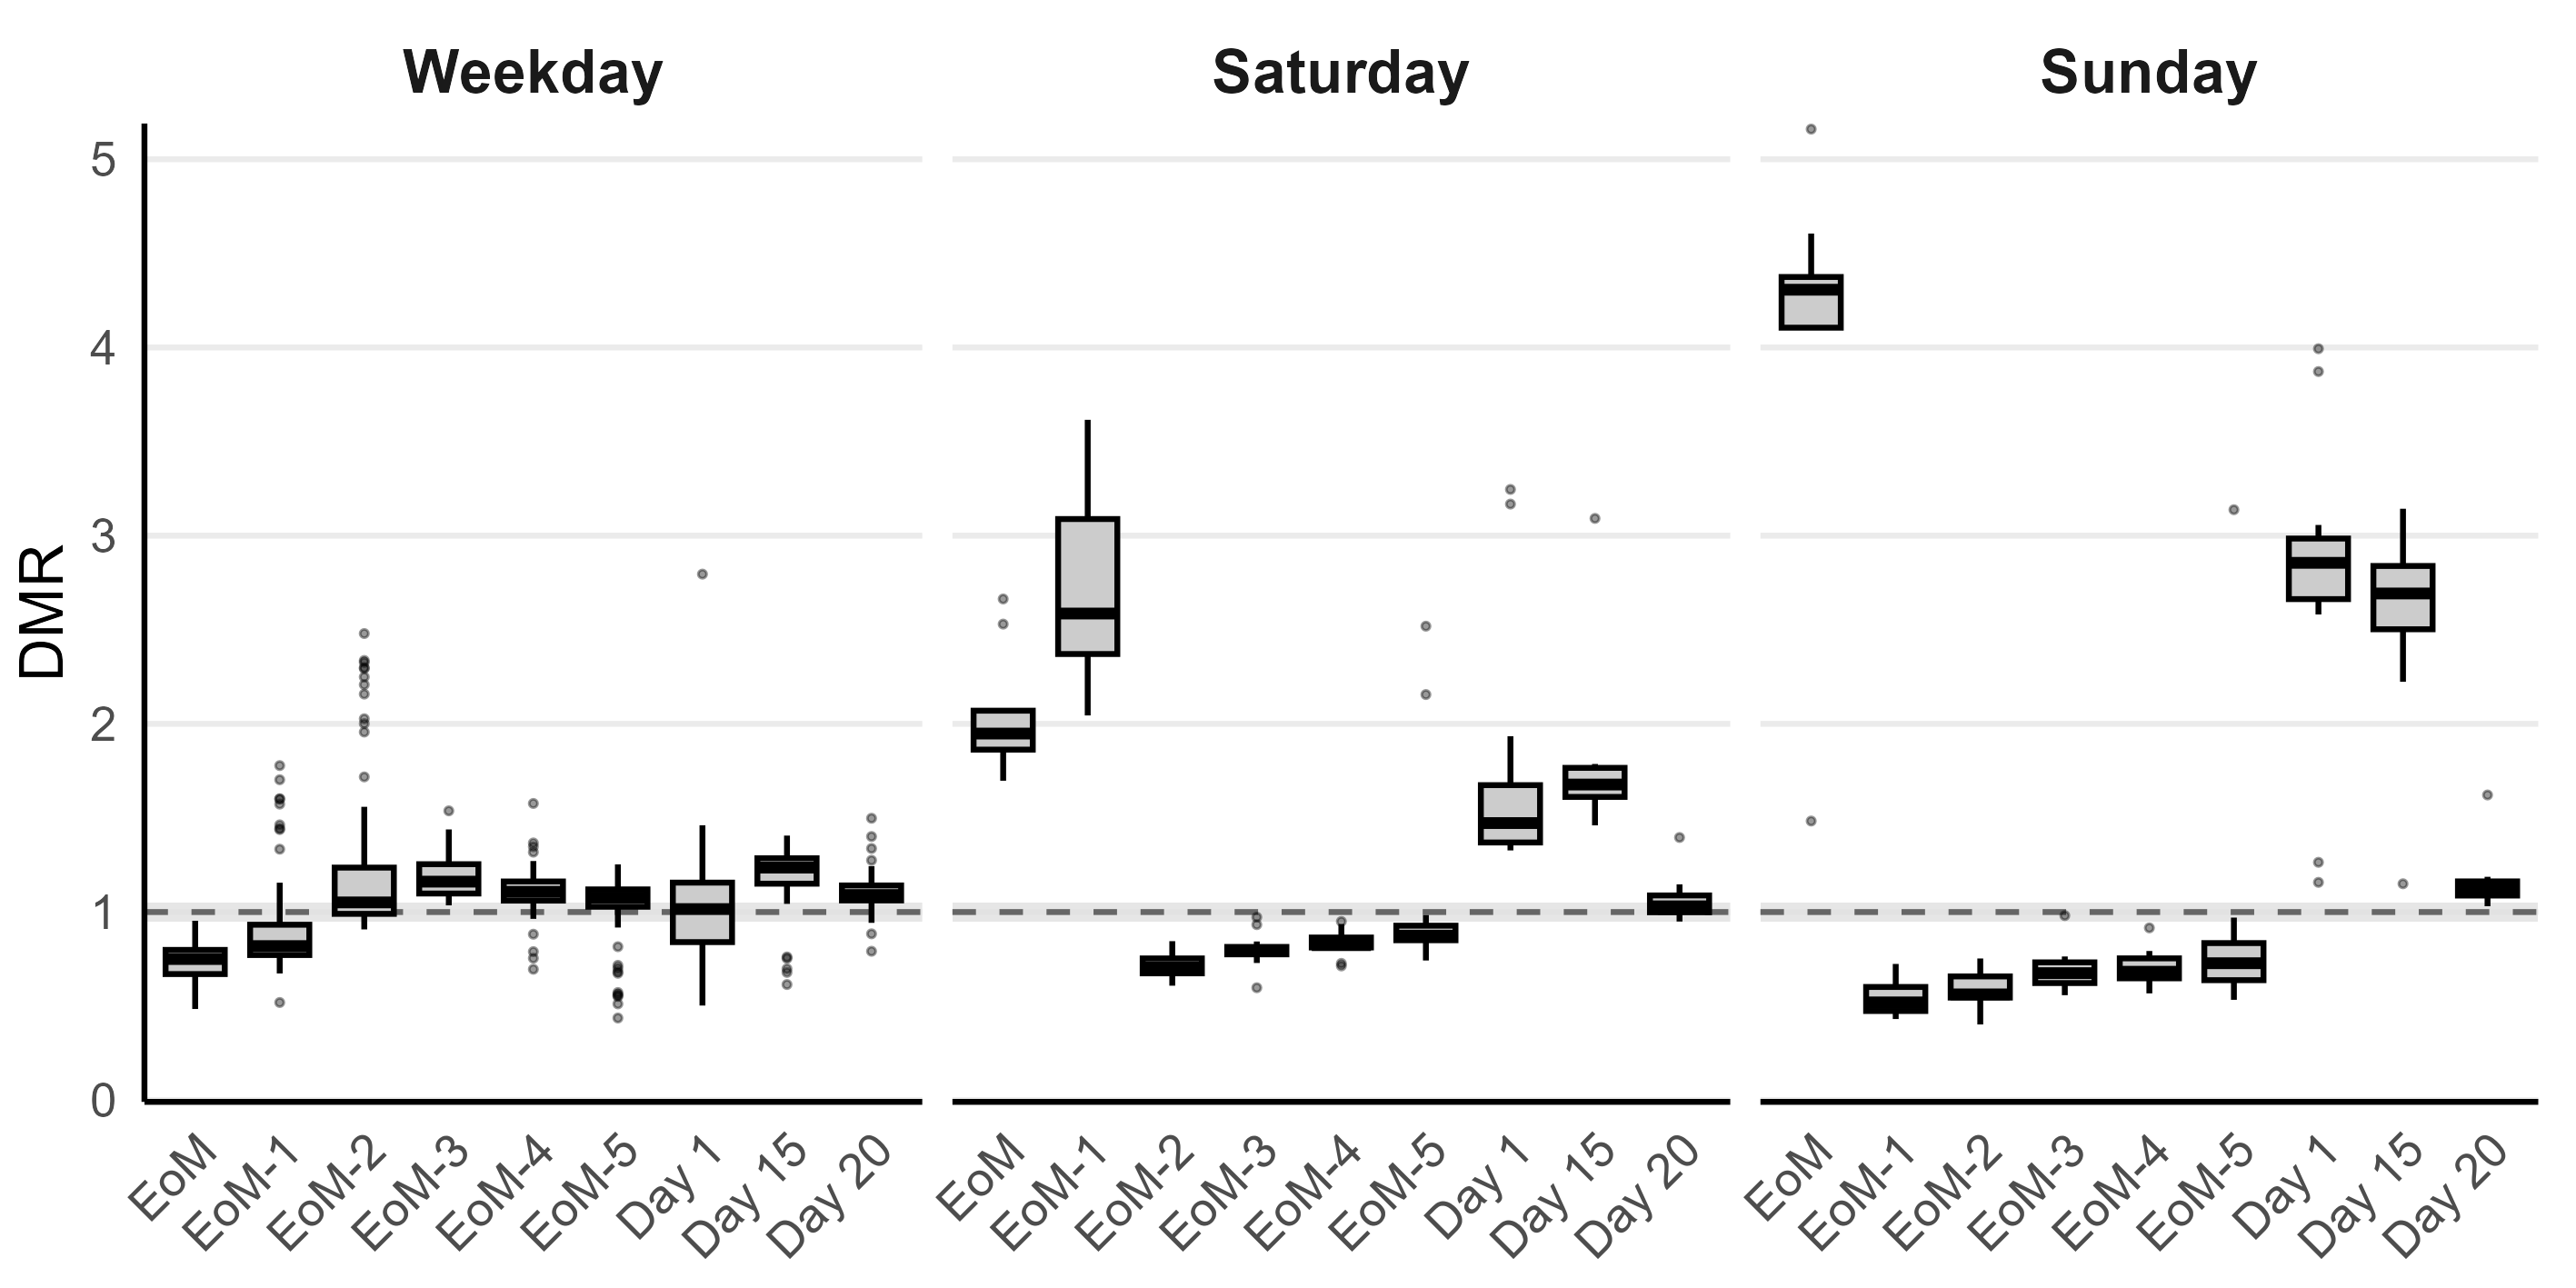
\includegraphics[width=0.95\textwidth]{figures/einv_dmr_day_type_basic.png}
\caption{E-invoicing, basic calendar: DMR on month-end and fixed days, split by type of day.}
\label{fig:einv_daytype}
\end{figure*}

Every month-end and fixed-day regressor is therefore split into weekday, Saturday and Sunday versions. The split also reveals an operational calendar that a purely technical count of days would miss. A weekend that is the month end is active, while a weekend that precedes a weekday month end is a normal weekend; and when the month ends on a weekend, invoicing moves to the last working day. A dedicated chart confirms the latter hypothesis: one and two days before the month end, Fridays had a median DMR of 1.46 and 2.2, against 0.81 and 1.03 for Monday to Thursday. A regressor for the Friday preceding a month end that falls on a weekend brings these groups between 0.99 and 1.04.

\subsection{The final calendar}

Holidays falling on Saturdays and Sundays are set to zero, so that a weekend holiday is treated as a normal weekend, except for Easter Sunday, which always falls on a Sunday and keeps its own effect relative to a normal Sunday. After this change the outliers fall from 13 to 8, and the residual on day 1 at weekends disappears, since New Year's Day, Labour Day and All Saints' Day on weekends had contaminated the estimates of the day-1 regressors. Month-end regressors are extended to the fifth day before the month end and day 20 is added. Finally, the calendar is simplified from 40 to 32 regressors: the Saturday regressors from two to five days before the month end are not significant ($t$ between \m0.7 and 0.3) and are dropped, showing that the pre-month-end ramp concerns working days only; the Sunday regressor one day before the month end, small and at the limit of significance, is also dropped; and the Sunday regressors from two to five days before the month end, with similar coefficients, are merged.

Table~\ref{tab:einv} reports the final pre-treatment model. On the multiplicative scale, the last day of the month is worth 8.6 normal weekdays, 30 normal Saturdays and 69 normal Sundays; the multipliers for days 1 and 15 range from 1.4 on weekdays to about 3.6--3.9 on Sundays; the ramp before the month end decreases from 1.44 one day before to 1.13 five days before. Weekend multipliers are relative to a normal weekend day, on which very few invoices are issued; they do not mean that more is invoiced on a Sunday month end than on a weekday month end. National holidays reduce invoicing to between 4\% (Christmas) and 31\% (Assumption Day) of a normal weekday; Easter Sunday is 0.67 times a normal Sunday. The remaining outliers are events: the 2020 lockdown (level shift of \m34\%) and the reopening (+32\%), other Covid-19 episodes, St.~Stephen's Day 2020 on a Saturday, and two first Sundays of February whose cause is still to be found. An additive outlier on 8 February 2025 treats a missing value.

\begin{table*}[t]
\centering
\caption{E-invoicing: final pre-treatment model (log scale).}
\label{tab:einv}
\footnotesize
\setlength{\tabcolsep}{4pt}
\resizebox{\textwidth}{!}{%
\begin{tabular}{@{}l r r@{\hspace{0.5cm}}l r r r@{}}
\toprule
\multicolumn{3}{@{}l}{\textit{A. National holidays}} & \multicolumn{4}{l@{}}{\textit{B. Month end and fixed days, coef.\ (t)}} \\
\cmidrule(r){1-3}\cmidrule(l){4-7}
 & Coef. & $t$ & & Weekday & Saturday & Sunday \\
\midrule
New Year's Day        & \m1.327 & \m16.3 & EoM    & 2.150 (71.0) & 3.388 (64.1) & 4.229 (85.3) \\
Epiphany              & \m2.070 & \m26.3 & EoM\m1 & 0.367 (11.9) & 1.809 (37.0) & -- \\
Easter Sunday$^{a}$   & \m0.394 & \m6.4  & EoM\m2 & 0.284 (9.4)  & --           & \multirow{4}{*}{\m0.204 (\m7.6)$^{b}$} \\
Easter Monday         & \m2.376 & \m38.7 & EoM\m3 & 0.282 (9.8)  & --           & \\
Liberation Day        & \m2.176 & \m26.4 & EoM\m4 & 0.195 (6.9)  & --           & \\
Labour Day            & \m1.518 & \m18.7 & EoM\m5 & 0.123 (4.5)  & --           & \\
Republic Day          & \m1.908 & \m23.1 & Day 1  & 0.341 (11.2) & 0.648 (13.3) & 1.351 (26.5) \\
Assumption of Mary    & \m1.160 & \m14.2 & Day 15 & 0.312 (12.9) & 0.755 (16.2) & 1.269 (26.1) \\
All Saints' Day       & \m1.609 & \m19.4 & Day 20 & 0.148 (6.3)  & 0.221 (4.9)  & 0.252 (5.4) \\
Immaculate Conception & \m1.843 & \m22.4 & Last working day$^{c}$ & 0.748 (20.6) & -- & -- \\
Christmas             & \m3.168 & \m38.0 & & & & \\
St.\ Stephen's Day    & \m2.771 & \m31.3 & & & & \\
\midrule
\multicolumn{3}{@{}l}{\textit{C. Model parameters}} & \multicolumn{4}{l@{}}{\textit{D. Outliers}} \\
\cmidrule(r){1-3}\cmidrule(l){4-7}
MA(1)                      & \m0.201 & \m10.2 & AO 03/02/2019 & 1.189 (7.4)    & \multicolumn{2}{l@{}}{First Sunday of February} \\
Seasonal MA, period 7      & 0.953   & 148.9  & AO 02/02/2020 & 1.157 (7.3)    & \multicolumn{2}{l@{}}{First Sunday of February} \\
Seasonal MA, period 365.24 & 0.837   & 65.1   & LS 09/03/2020 & \m0.414 (\m15.1) & \multicolumn{2}{l@{}}{Covid-19 lockdown} \\
 & & & AO 05/04/2020 & 1.041 (6.6)    & \multicolumn{2}{l@{}}{Covid-19 period} \\
 & & & LS 02/06/2020 & 0.281 (10.3)   & \multicolumn{2}{l@{}}{End of lockdown} \\
 & & & WO 06/12/2020 & 0.636 (6.2)    & \multicolumn{2}{l@{}}{Covid-19 period} \\
 & & & AO 26/12/2020 & \m1.101 (\m6.8)  & \multicolumn{2}{l@{}}{St.\ Stephen's Day on Saturday} \\
\bottomrule
\end{tabular}}
\begin{minipage}{\textwidth}
\footnotesize
\vspace{4pt}
Notes: 2,557 observations (2019--2025), 32 calendar regressors, all with $|t| > 4$; the multiplicative effect is exp(coefficient). Holidays enter only when they fall on a working day. Effects in panel B are relative to a normal day of the same type. EoM: last day of the month; EoM\m$k$: $k$ days before. -- not included (not significant). An additional AO on 08/02/2025 treats a missing value and is not reported. $^{a}$~Relative to a normal Sunday. $^{b}$~Single regressor for Sundays falling 2 to 5 days before the month end. $^{c}$~Friday before a month end falling on a weekend, added to the EoM\m1 or EoM\m2 weekday effect.
\end{minipage}
\end{table*}

With the final calendar, the median DMR by day of the month is within $\pm5\%$ on every day except days 2 and 9 (0.95 and 0.94), which we leave as minor residuals: day 1 moves from 1.13 to 0.99, day 15 from 1.27 to 1.01 and day 31 from 0.76 to 1.00 (Figure~\ref{fig:einv_final}). The boxes also become much narrower, especially at the end of the month. Of the 27 cells defined by the special days with a dedicated regressor and the three types of day, 26 are within the tolerance; the last one, Sundays falling five days before the month end, is at 0.946.

\begin{figure*}[t]
\centering
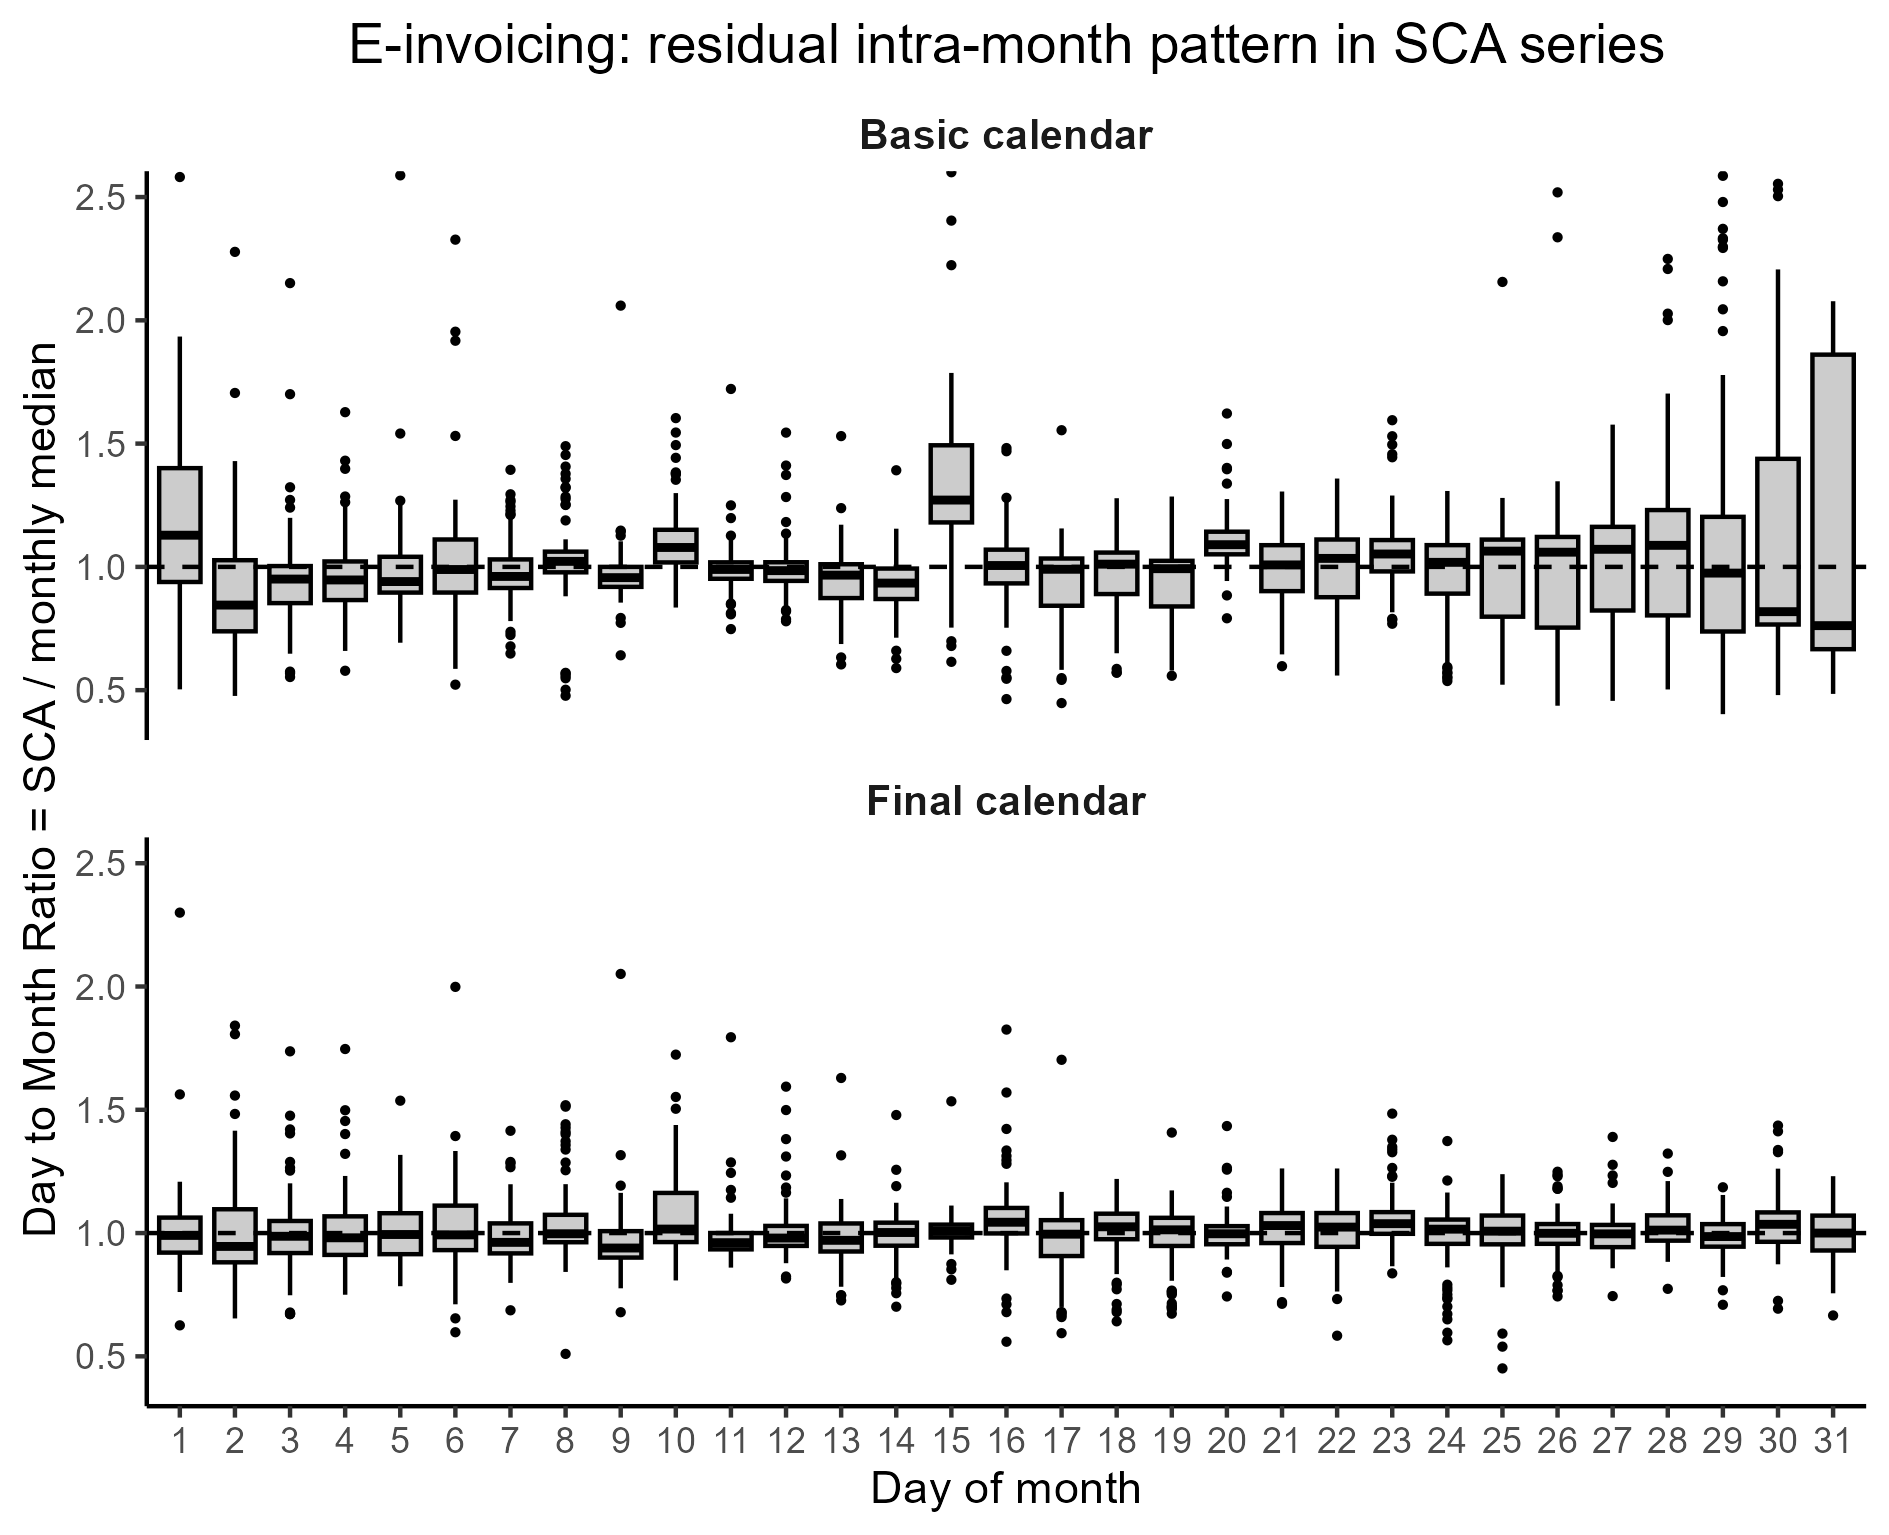
\includegraphics[width=0.85\textwidth]{figures/einv_dmr_day_of_month_basic_final.png}
\caption{E-invoicing: DMR by day of the month with the basic calendar (top) and the final calendar (bottom), on the same scale.}
\label{fig:einv_final}
\end{figure*}

We also estimated the calendar with time-varying coefficients (Section~\ref{subsec:tv}). The estimated variance of the coefficients was zero, so that the coefficients were in fact constant; moreover, the flexible local level of the preliminary model absorbed gradual effects such as the pre-month-end ramp, which the dummies could no longer capture. The e-invoicing calendar is therefore estimated with fixed coefficients, jointly with the pre-treatment model.

% =============================================================================
\section{Electricity demand: a production calendar}
\label{sec:el}

\subsection{Building the calendar}

The diagnostic transfers from e-invoicing, but the calendar does not. For electricity demand, the DMR profiles by day of the week, day of the month and days to the end of the month are flat already with the basic calendar (median DMR between 0.996 and 1.004): there are no intra-month effects, and no month-end or fixed-day regressors are needed. The relevant effects are those of a production calendar, driven by plant activity and closures.

\textit{Holidays by type of day.} With holidays active on every day, holidays on Saturdays and Sundays are over-corrected (median DMR 1.085 and 1.022) and holidays on Tuesdays and Wednesdays under-corrected (0.927 and 0.935). In an additive model a holiday effect is a quantity of MWh, and the same quantity cannot be removed from a weekday and from a Sunday, when demand is already low. Holidays are therefore active from Monday to Friday only. A holiday on a Saturday is still lower than a normal Saturday and gets a single regressor; and a holiday on Tuesday to Thursday starts from the highest weekly level, which motivates an additional midweek effect.

\textit{Bridges.} The DMR around holidays, split by the weekday of the holiday, shows the bridges: the Monday before a Tuesday holiday has a median DMR of 0.905, the Friday after a Thursday holiday 0.914, while the days around holidays falling on other weekdays are close to 1. Two bridge regressors are added.

\textit{Semi-closure days.} Christmas Eve and New Year's Eve, the working days between Christmas and Epiphany, and 14 and 16 August have fixed dates, but their effect exists only on working days. The annual seasonal component can capture only their average effect across years, so that, with the basic calendar, these dates are under-corrected when they fall on weekdays (24 December: 0.919) and artificially corrected when they fall at weekends (up to 1.082). They are modelled with regressors active on working days only.

\textit{The Easter window.} The drop in demand extends from Good Friday to the Tuesday after Easter Monday (median DMR between 0.938 and 0.976 with the basic calendar). Modelling the whole window also improves Easter Sunday and Easter Monday, which already had their own regressors: a drop over several days that is not modelled is partly absorbed by the local level of the model, which biases the effects of the modelled days towards zero.

The final calendar has 23 regressors: eleven national holidays on working days and Easter Sunday, two bridge regressors, four semi-closure regressors, the Saturday holiday, Good Friday, Holy Saturday, Easter Tuesday and the midweek effect.

\subsection{Time-varying coefficients}

Holiday effects on electricity demand change over time, and the calendar is estimated with time-varying coefficients (Section~\ref{subsec:tv}). The decision required care. In the original specification, with holidays active also at weekends, the range of the coefficients over the sample was 135--190 thousand MWh; once weekend holidays were set to zero it fell to 17--42 thousand MWh. Most of the apparent variation was therefore an artefact: free coefficients absorb specification errors, for instance an All Saints' Day on a Saturday at the end of the sample pulled the coefficient from \m154 to \m54 thousand MWh. With the complete calendar, however, a gradual and common drift remains. Fixed and time-varying coefficients perform similarly on the DMR: the time-varying model is better on midweek holidays (median DMR 0.977 against 0.960--0.965) and bridges (1.000 and 0.993 against 0.993 and 0.987), the fixed model on the Easter window (0.988--0.995 against 0.977--0.983). The two adjusted series differ by less than 0.2\% on most days and by 3--4\% on the holidays of 2024--2025, where the time-varying coefficients use current values instead of a fourteen-year average. We retain time-varying coefficients, consistent with the observed drift. \todo{report the likelihood-ratio statistic for $\sigma^2_\xi = 0$}

Figure~\ref{fig:el_tv} shows the smoothed coefficients. National holiday effects weaken gradually, mostly after 2018: between the end of 2012 and the end of 2025 the effect of Republic Day moves from \m174 to \m143 thousand MWh, that of Easter Monday from \m221 to \m198, and only Assumption Day is broadly stable (\m132 to \m128). Bridges and semi-closure days do not fade, and some strengthen: the Monday bridge moves from \m52 to \m77 thousand MWh, New Year's Eve on a working day from \m76 to \m97. Saturday holidays weaken (\m73 to \m55), while the Tuesday after Easter Monday strengthens (\m30 to \m46). The midweek effect moves from \m21 to +2, but it overlaps with the individual holiday regressors: the two paths can offset each other, and only their sum is meaningful. The causes of the drift are an open question; a lower industrial share of consumption and self-generation from rooftop solar are hypotheses worth investigating.

\begin{figure*}[t]
\centering
\begin{subfigure}{0.6\textwidth}
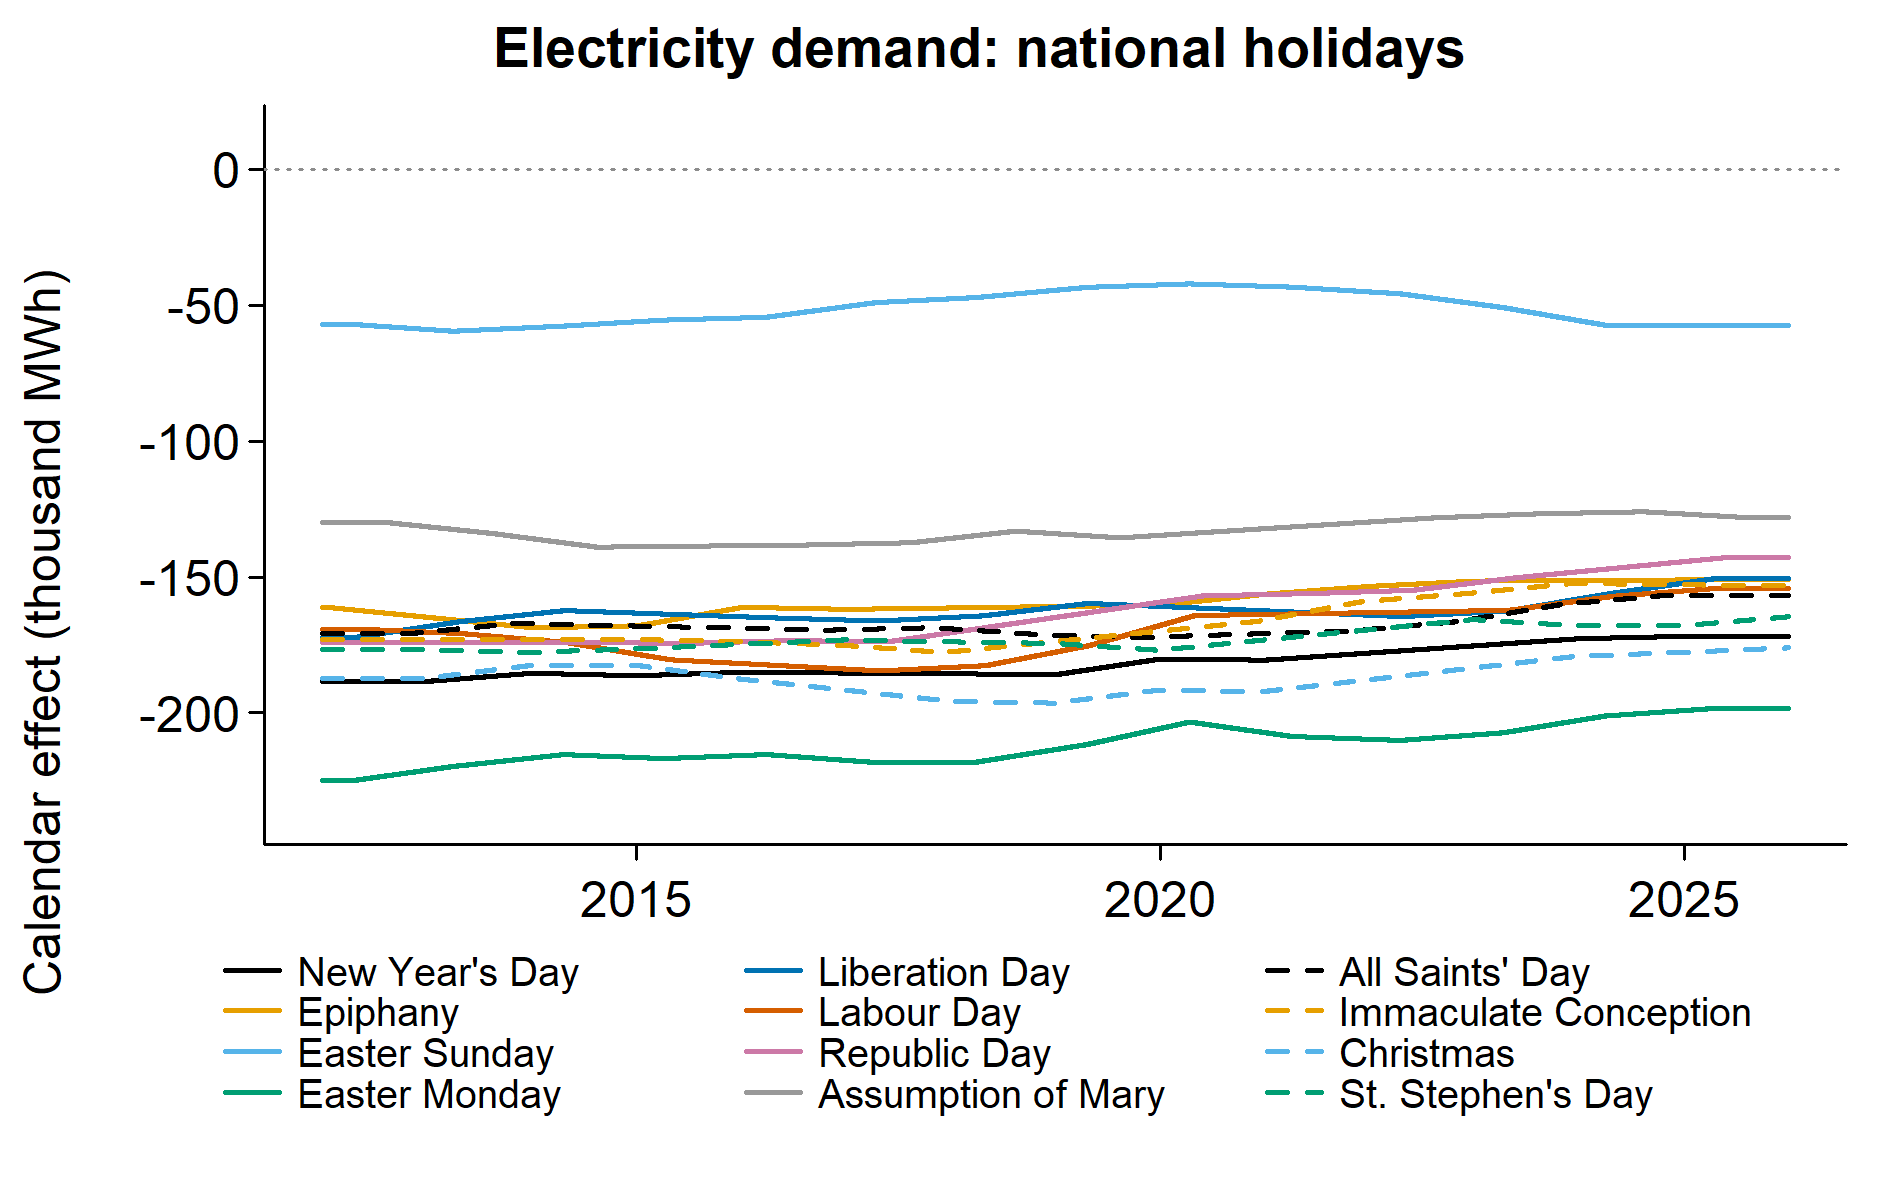
\includegraphics[width=\linewidth]{figures/el_tv_holidays.png}
\caption{National holidays}
\end{subfigure}

\begin{subfigure}{0.6\textwidth}
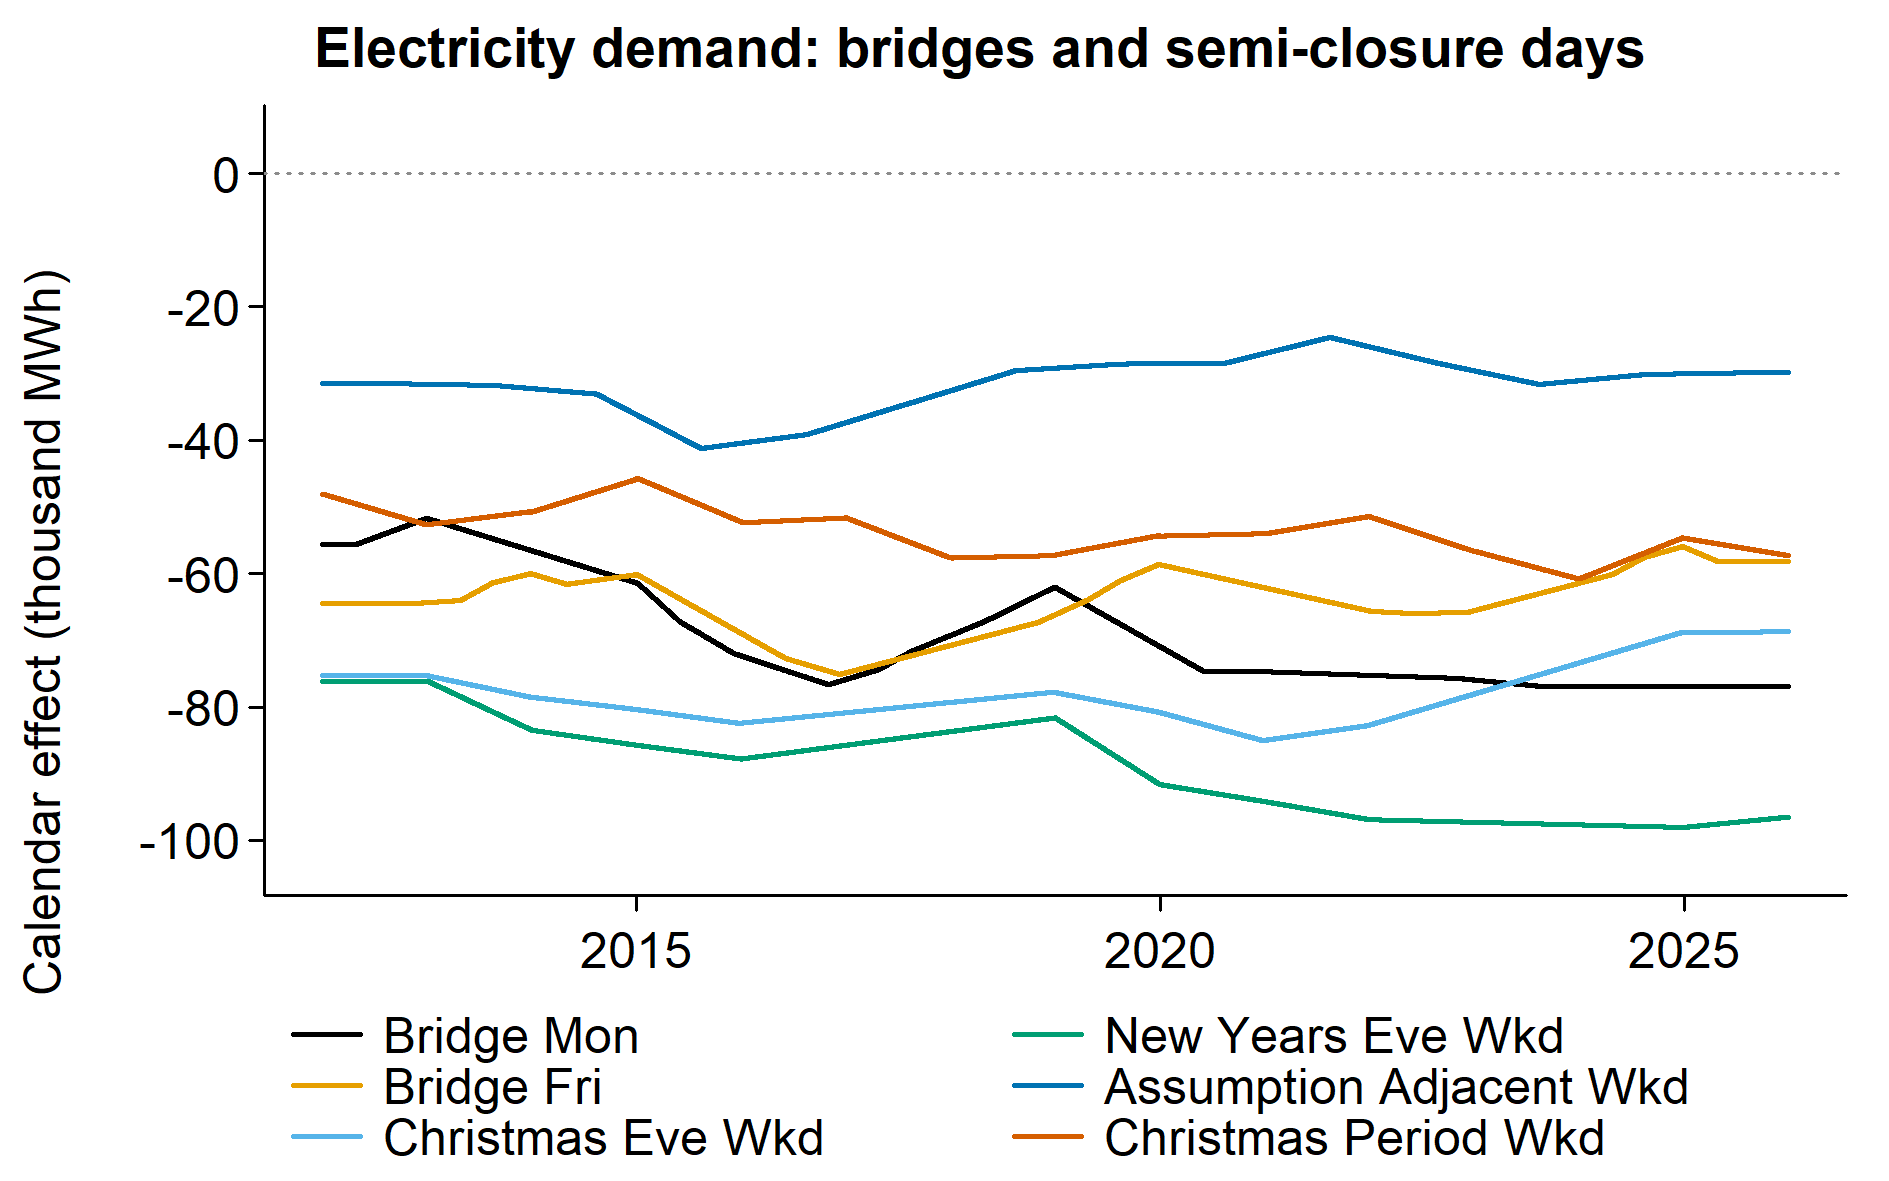
\includegraphics[width=\linewidth]{figures/el_tv_bridges.png}
\caption{Bridges and semi-closure days}
\end{subfigure}

\begin{subfigure}{0.6\textwidth}
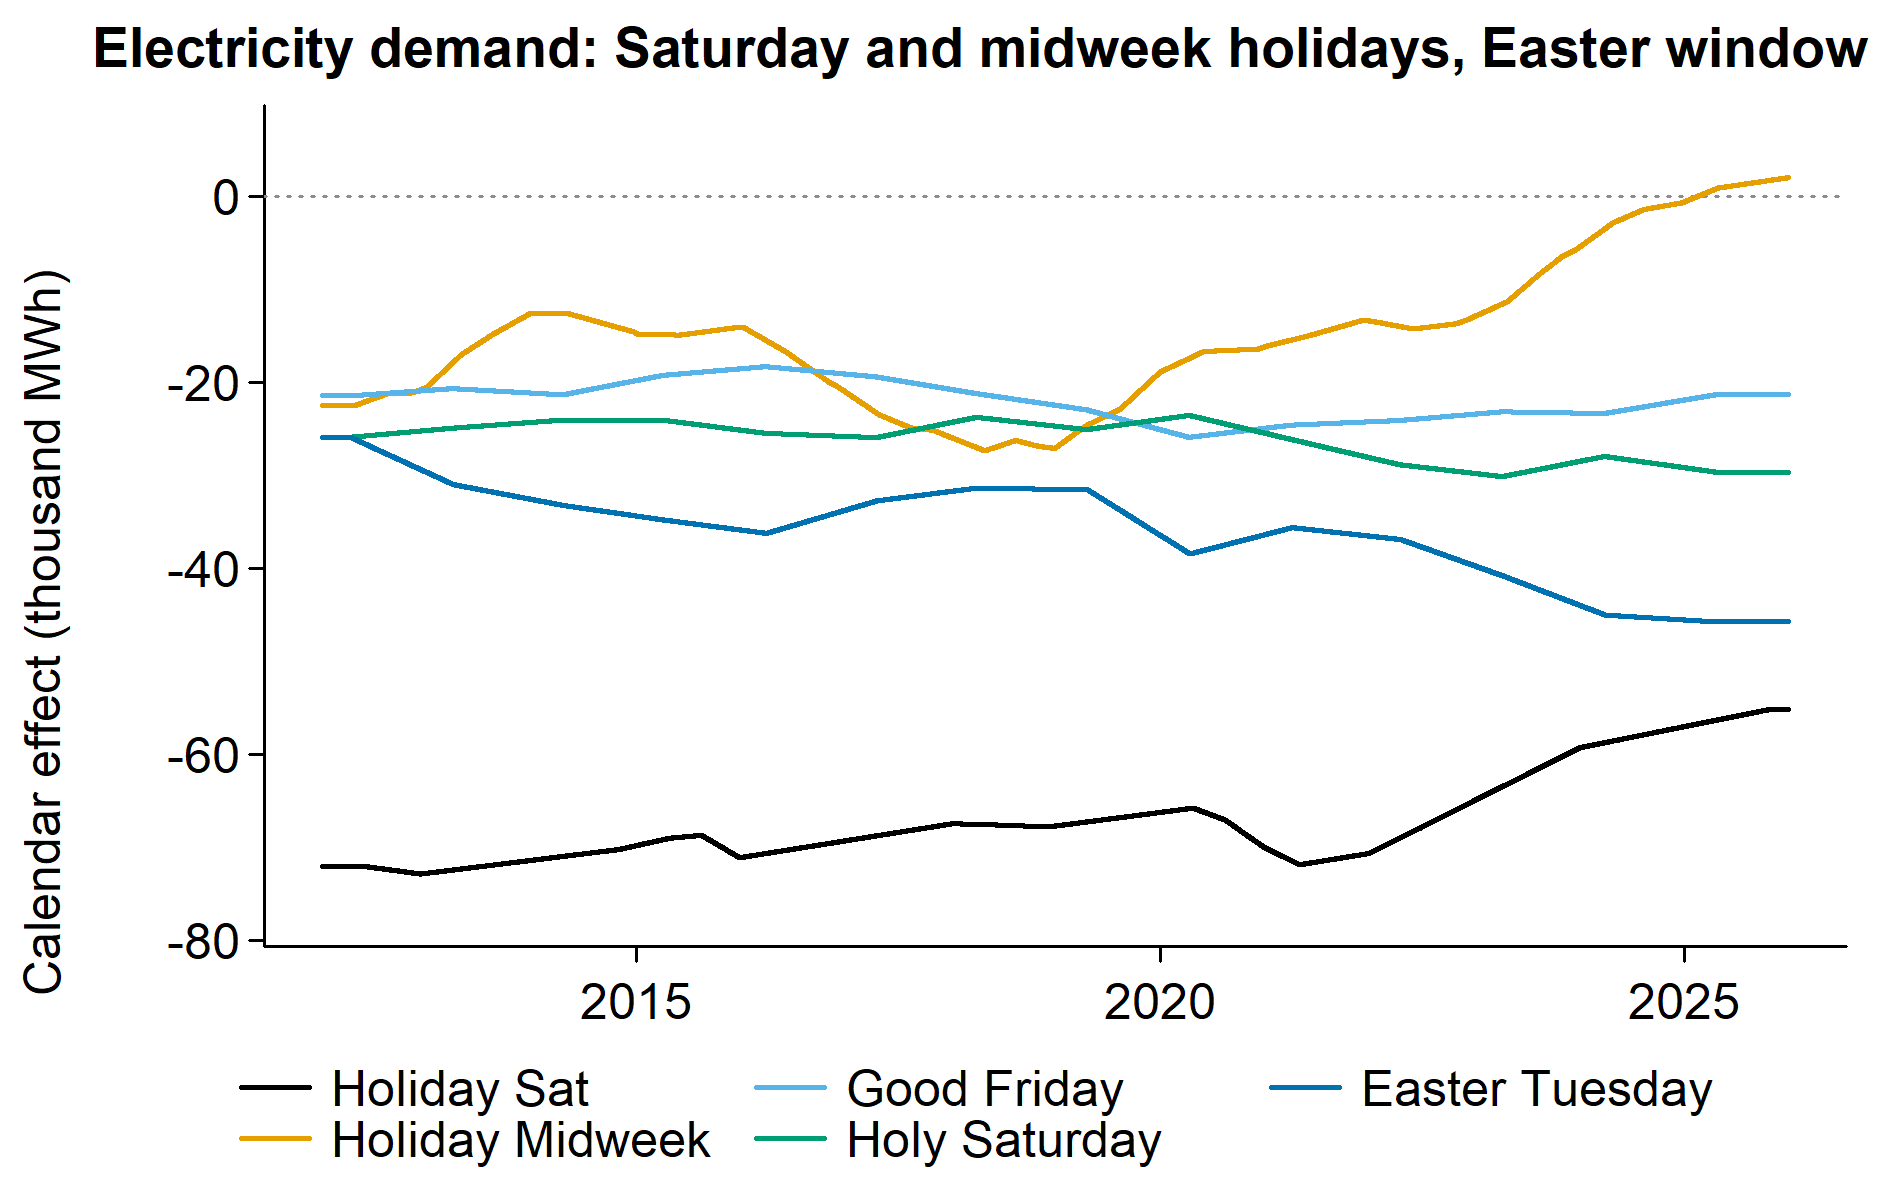
\includegraphics[width=\linewidth]{figures/el_tv_other.png}
\caption{Saturday and midweek holidays, Easter window}
\end{subfigure}
\caption{Electricity demand: smoothed time-varying calendar coefficients, 2012--2025 (thousand MWh).}
\label{fig:el_tv}
\end{figure*}

\subsection{Results}

Table~\ref{tab:el_dmr} compares the median DMR on the special days with the two calendars. With the basic calendar, 7 of the 14 groups are outside the tolerance; with the final calendar only one is, 14 and 16 August on working days (0.949), discussed in Section~\ref{sec:discussion}. Figure~\ref{fig:el_dmr} shows the whole distributions: the boxes move towards 1 and become narrower. Over the Christmas period, by date and type of day, the groups outside the tolerance fall from 13 to none of 38.

\begin{table*}[t]
\centering
\caption{Electricity demand: median DMR on special days, basic and final calendar.}
\label{tab:el_dmr}
\small
\begin{tabular}{@{}l r r r@{}}
\toprule
Group of days & Days & Basic calendar & Final calendar \\
\midrule
Holiday, Monday to Friday    & 103 & 0.953 & 0.982 \\
Holiday on Saturday          & 17  & \textbf{1.085} & 1.005 \\
Holiday on Sunday            & 20  & 1.022 & 0.990 \\
Monday bridge                & 17  & \textbf{0.914} & 1.000 \\
Friday bridge                & 19  & \textbf{0.928} & 0.993 \\
24 December, working day     & 8   & \textbf{0.925} & 0.963 \\
31 December, working day     & 8   & \textbf{0.937} & 0.976 \\
Christmas period, working days & 74 & 0.971 & 0.984 \\
14 and 16 August, working days & 16 & \textbf{0.941} & \textbf{0.949} \\
Good Friday                  & 14  & 0.976 & 0.994 \\
Holy Saturday                & 14  & 0.958 & 0.989 \\
Easter Sunday                & 14  & 0.972 & 0.983 \\
Easter Monday                & 14  & 0.955 & 0.978 \\
Easter Tuesday               & 14  & \textbf{0.938} & 0.977 \\
\bottomrule
\end{tabular}
\begin{minipage}{0.75\textwidth}
\footnotesize
\vspace{4pt}
Notes: each day belongs to one group only. In bold: outside $1\pm0.05$. Basic calendar: twelve national holidays active on every day, fixed coefficients. Final calendar: 23 regressors with time-varying coefficients.
\end{minipage}
\end{table*}

\begin{figure*}[t]
\centering
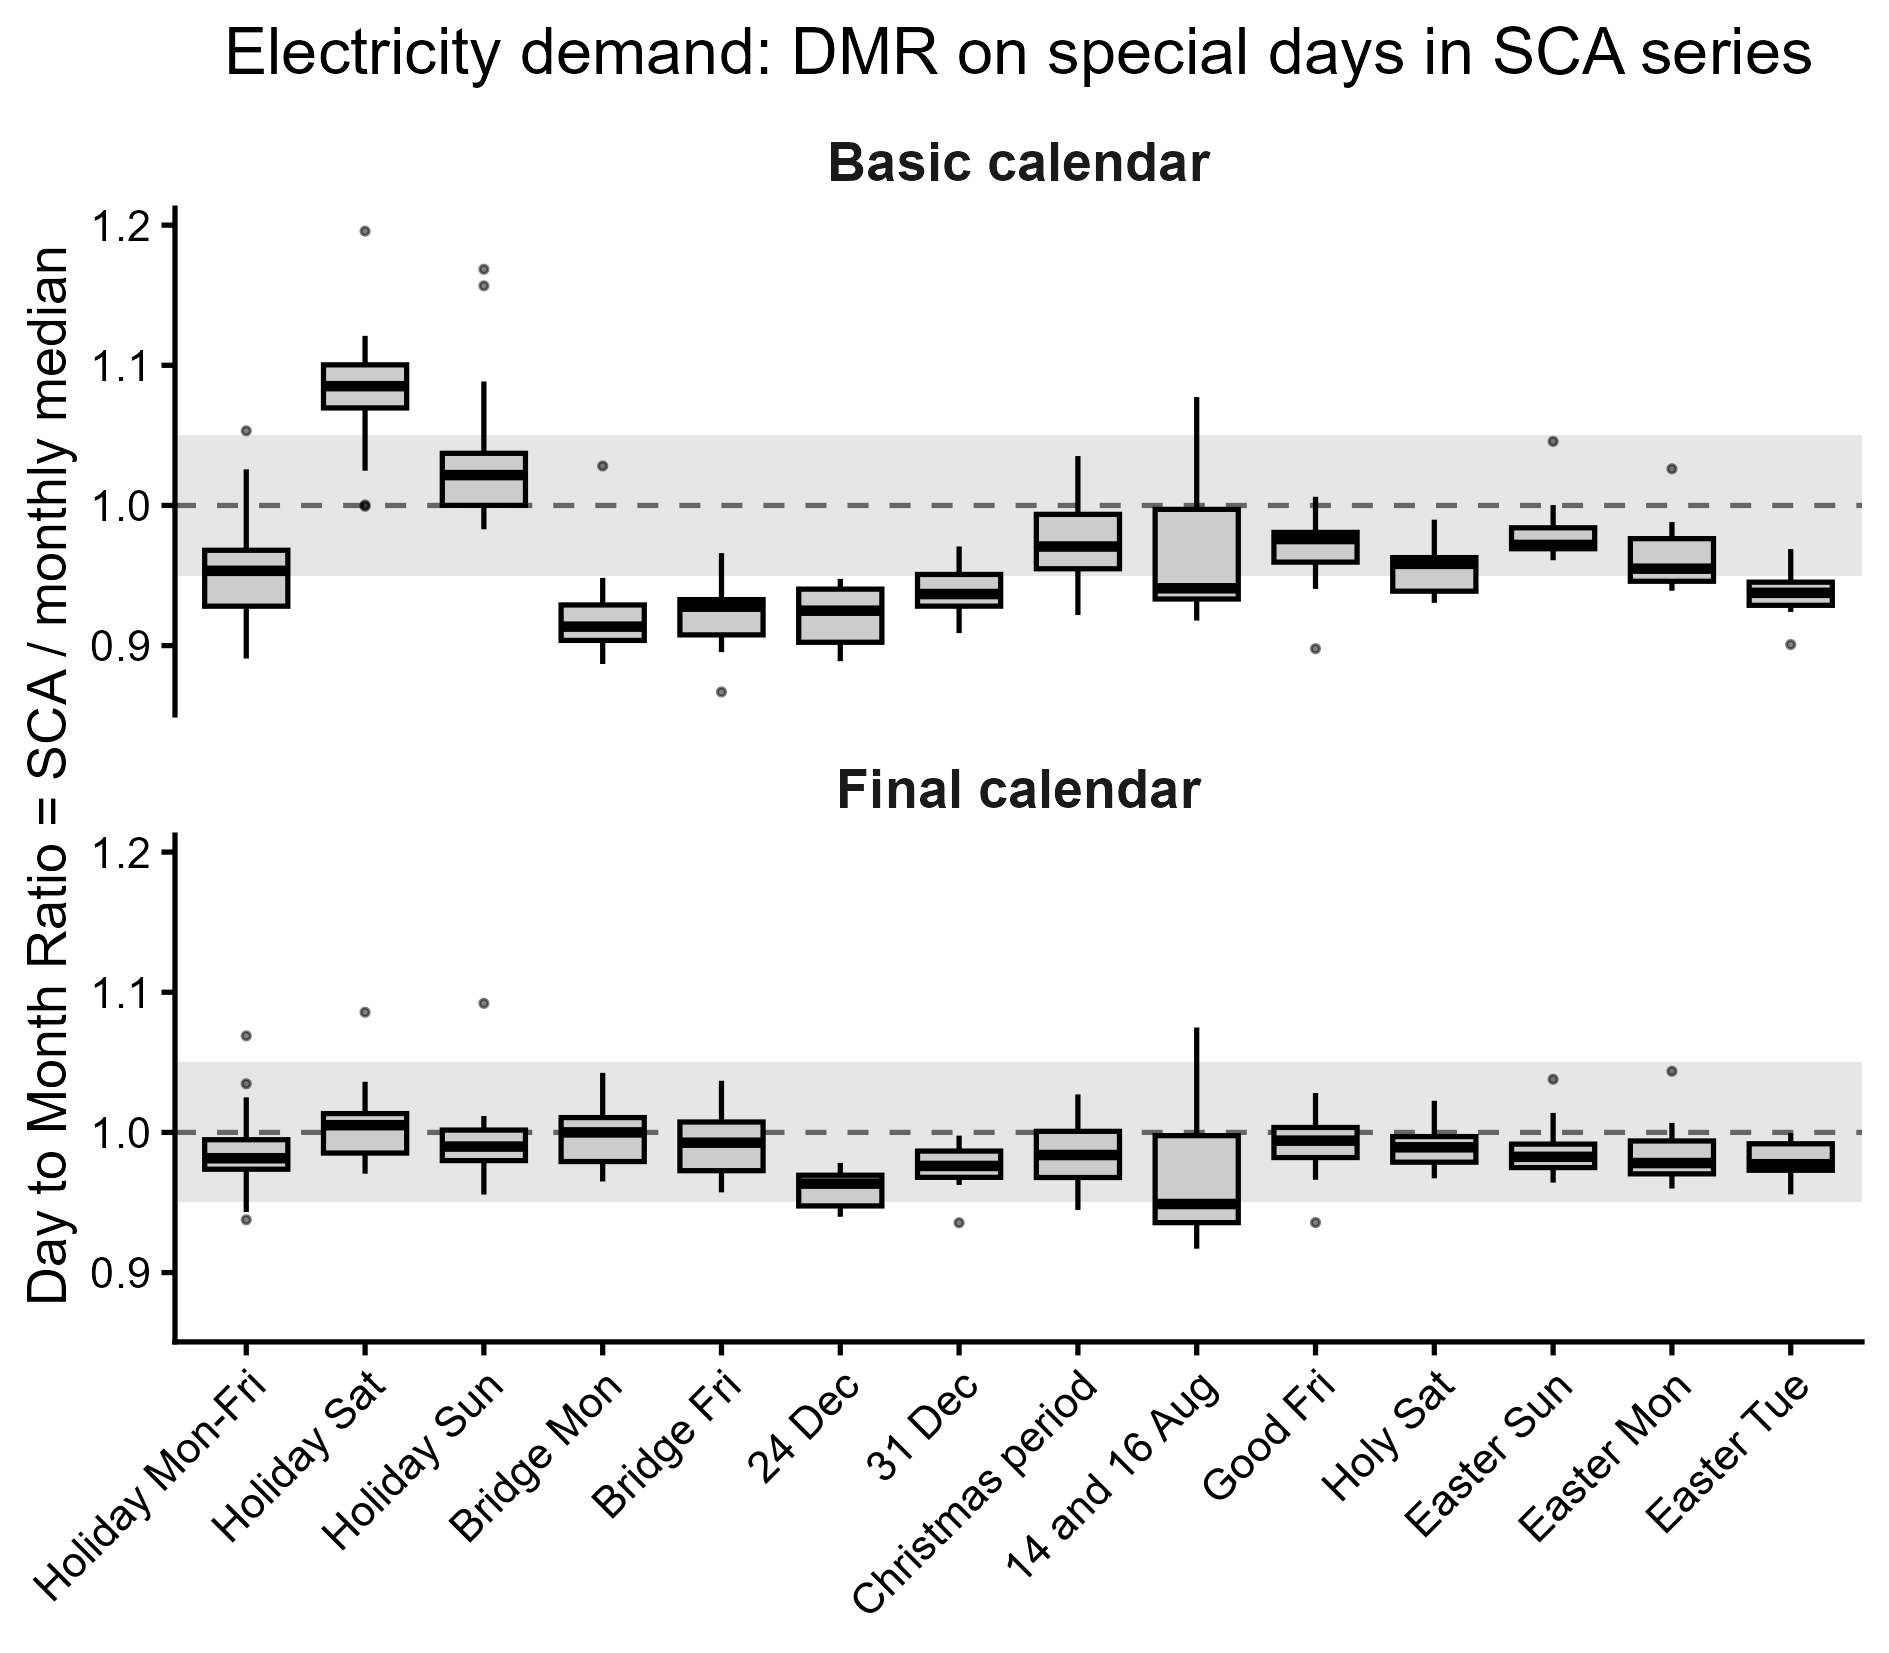
\includegraphics[width=0.8\textwidth]{figures/el_dmr_special_days_basic_final.png}
\caption{Electricity demand: DMR on special days with the basic calendar (top) and the final calendar (bottom), on the same scale.}
\label{fig:el_dmr}
\end{figure*}

Table~\ref{tab:el_pre} reports the pre-treatment of the calendar-adjusted series. Of the 15 outliers, four are economic events (the 2020 lockdown and two reopening phases, and the 2022 energy crisis) and ten are summer level shifts, mostly in pairs of opposite sign, which point to temperature effects that are not modelled. The additive outlier on 21 August 2015 coincides with a storm and a sharp drop in temperature, which cut cooling demand for a day: like the summer level shifts, it points to weather effects that the calendar cannot capture.

\begin{table*}[t]
\centering
\caption{Electricity demand: pre-treatment of the calendar-adjusted series (additive model).}
\label{tab:el_pre}
\footnotesize
\setlength{\tabcolsep}{4pt}
\resizebox{\textwidth}{!}{%
\begin{tabular}{@{}l r r@{\hspace{0.5cm}}l l r r l@{}}
\toprule
\multicolumn{3}{@{}l}{\textit{A. Model parameters}} & \multicolumn{5}{l@{}}{\textit{B. Outliers (thousand MWh)}} \\
\cmidrule(r){1-3}\cmidrule(l){4-8}
 & Coef. & $t$ & Type & Date & Coef. & $t$ & Event \\
\midrule
MA(1)                      & \m0.707 & \m82.6 & LS & 15/06/2014 & \m51.4  & \m10.0 & Summer temperature \\
Seasonal MA, period 7      & 0.869   & 81.2   & LS & 01/09/2014 & 41.6    & 8.1    & Summer temperature \\
Seasonal MA, period 365.24 & 0.889   & 150.0  & AO & 21/08/2015 & \m71.4  & \m6.5  & Storm, sharp temperature drop \\
 & & & LS & 29/08/2016 & 32.0    & 6.4    & Summer temperature \\
 & & & LS & 15/03/2020 & \m131.9 & \m24.1 & Covid-19 lockdown \\
 & & & LS & 25/04/2020 & 68.5    & 12.4   & Covid-19 reopening \\
 & & & LS & 27/07/2020 & 66.8    & 13.2   & Covid-19 reopening \\
 & & & LS & 22/08/2022 & \m42.4  & \m8.4  & Energy crisis \\
 & & & LS & 10/07/2023 & 75.2    & 10.8   & Summer temperature \\
 & & & LS & 26/07/2023 & \m94.1  & \m12.1 & Summer temperature \\
 & & & LS & 19/08/2023 & 53.2    & 8.5    & Summer temperature \\
 & & & LS & 09/07/2024 & 79.3    & 15.0   & Summer temperature \\
 & & & LS & 10/09/2024 & \m61.7  & \m11.7 & Summer temperature \\
 & & & LS & 04/06/2025 & 55.5    & 9.6    & Summer temperature \\
 & & & LS & 08/07/2025 & \m45.8  & \m7.8  & Summer temperature \\
\bottomrule
\end{tabular}}
\begin{minipage}{\textwidth}
\footnotesize
\vspace{4pt}
Notes: 5,114 observations (2012--2025). Calendar effects (23 regressors, time-varying coefficients) are removed in a first step; the fractional airline model with periods 7 and 365.2425 is then estimated on the calendar-adjusted series, with outlier detection (critical value 6).
\end{minipage}
\end{table*}

% =============================================================================
\section{Calendars and revisions}
\label{sec:rev}

A calendar that fits the historical series well may still behave poorly in real time, when the most recent special days are estimated at the end of the sample. We therefore compare the revisions of the SCA series obtained with the basic and the final calendars, for both series.

For each specification, the estimates on the full sample, ending on 31 December 2025, are compared with six vintages ending 7, 30, 90, 181, 365 and 730 days earlier (on 24/12/2025, 01/12/2025, 02/10/2025, 03/07/2025, 31/12/2024 and 01/01/2024). Each vintage repeats the whole procedure, including the automatic detection of outliers; the calendar regressors are known in advance and are simply truncated. Let $\SACA_{t|v}$ be the estimate for day $t$ from the vintage ending on day $v$, and $T$ the end of the full sample. We compute the relative mean absolute revision
\begin{equation}
\mathrm{RMAR} = \frac{100}{|S|} \sum_{t \in S} \frac{\left|\SACA_{t|T} - \SACA_{t|v}\right|}{\SACA_{t|T}}
\end{equation}
over two sets of days $S$: a common historical sample, up to the end of the oldest vintage (1 January 2024), and the last 365 days of each vintage, separately for the special days of each series and for the other days. The first measure describes the stability of the historical series; the second, the revisions of the most recent data, where calendar effects are estimated with the least information.

\subsection{Electricity demand}
\label{subsec:rev_el}

For electricity we compare four specifications that cross the two calendars with the two estimation approaches (Table~\ref{tab:rev_el}): the basic calendar with fixed coefficients (A), the final calendar with fixed coefficients (B), the final calendar with time-varying coefficients (C, the adopted specification) and the basic calendar with time-varying coefficients (D). Comparing A with B, and D with C, measures the effect of the content of the calendar; comparing A with D, and B with C, the effect of time-varying coefficients. Special days are the holidays on any day of the week, bridges, semi-closure days and the Easter window, about 24 per year.

\begin{table*}[t]
\centering
\caption{Electricity demand: revisions of the SCA series under four specifications (RMAR, \%, mean over six vintages) and outliers in the full-sample model.}
\label{tab:rev_el}
\small
\begin{tabular}{@{}l l l r r r r r@{}}
\toprule
 & & & Historical & \multicolumn{3}{c}{Last year of each vintage} & Outliers \\
\cmidrule(lr){5-7}
 & Calendar & Coefficients & sample & All days & Special days & Other days & (on special days) \\
\midrule
A & Basic   & Fixed        & 0.145 & 0.219 & 0.503 & 0.199 & 28 (23) \\
B & Final   & Fixed        & 0.144 & 0.174 & 0.186 & 0.173 & 8 (1) \\
C & Final   & Time-varying & 0.121 & 0.153 & 0.229 & 0.148 & 15 (1) \\
D & Basic   & Time-varying & 0.161 & 0.218 & 0.308 & 0.212 & 9 (0) \\
\bottomrule
\end{tabular}
\begin{minipage}{\textwidth}
\footnotesize
\vspace{4pt}
Notes: basic calendar: twelve national holidays active on every day; final calendar: 23 regressors (Section~\ref{sec:el}). Vintages end on 24/12/2025, 01/12/2025, 02/10/2025, 03/07/2025, 31/12/2024 and 01/01/2024. Historical sample: days up to 01/01/2024, common to all vintages. The outlier on a special day in B and C is the level shift of 25/04/2020 (Covid-19 reopening), on a Liberation Day falling on a Saturday.
\end{minipage}
\end{table*}

On the historical sample the four specifications are close, with RMAR between 0.12\% and 0.16\% and the adopted specification C slightly ahead. The differences appear at the end of the sample and on special days (Figure~\ref{fig:rev_el}). Moving from the basic to the final calendar reduces the revisions of special days from 0.50\% to 0.19\% with fixed coefficients ($-63\%$) and from 0.31\% to 0.23\% with time-varying coefficients ($-26\%$), while the revisions of the other days change much less.

\begin{figure*}[t]
\centering
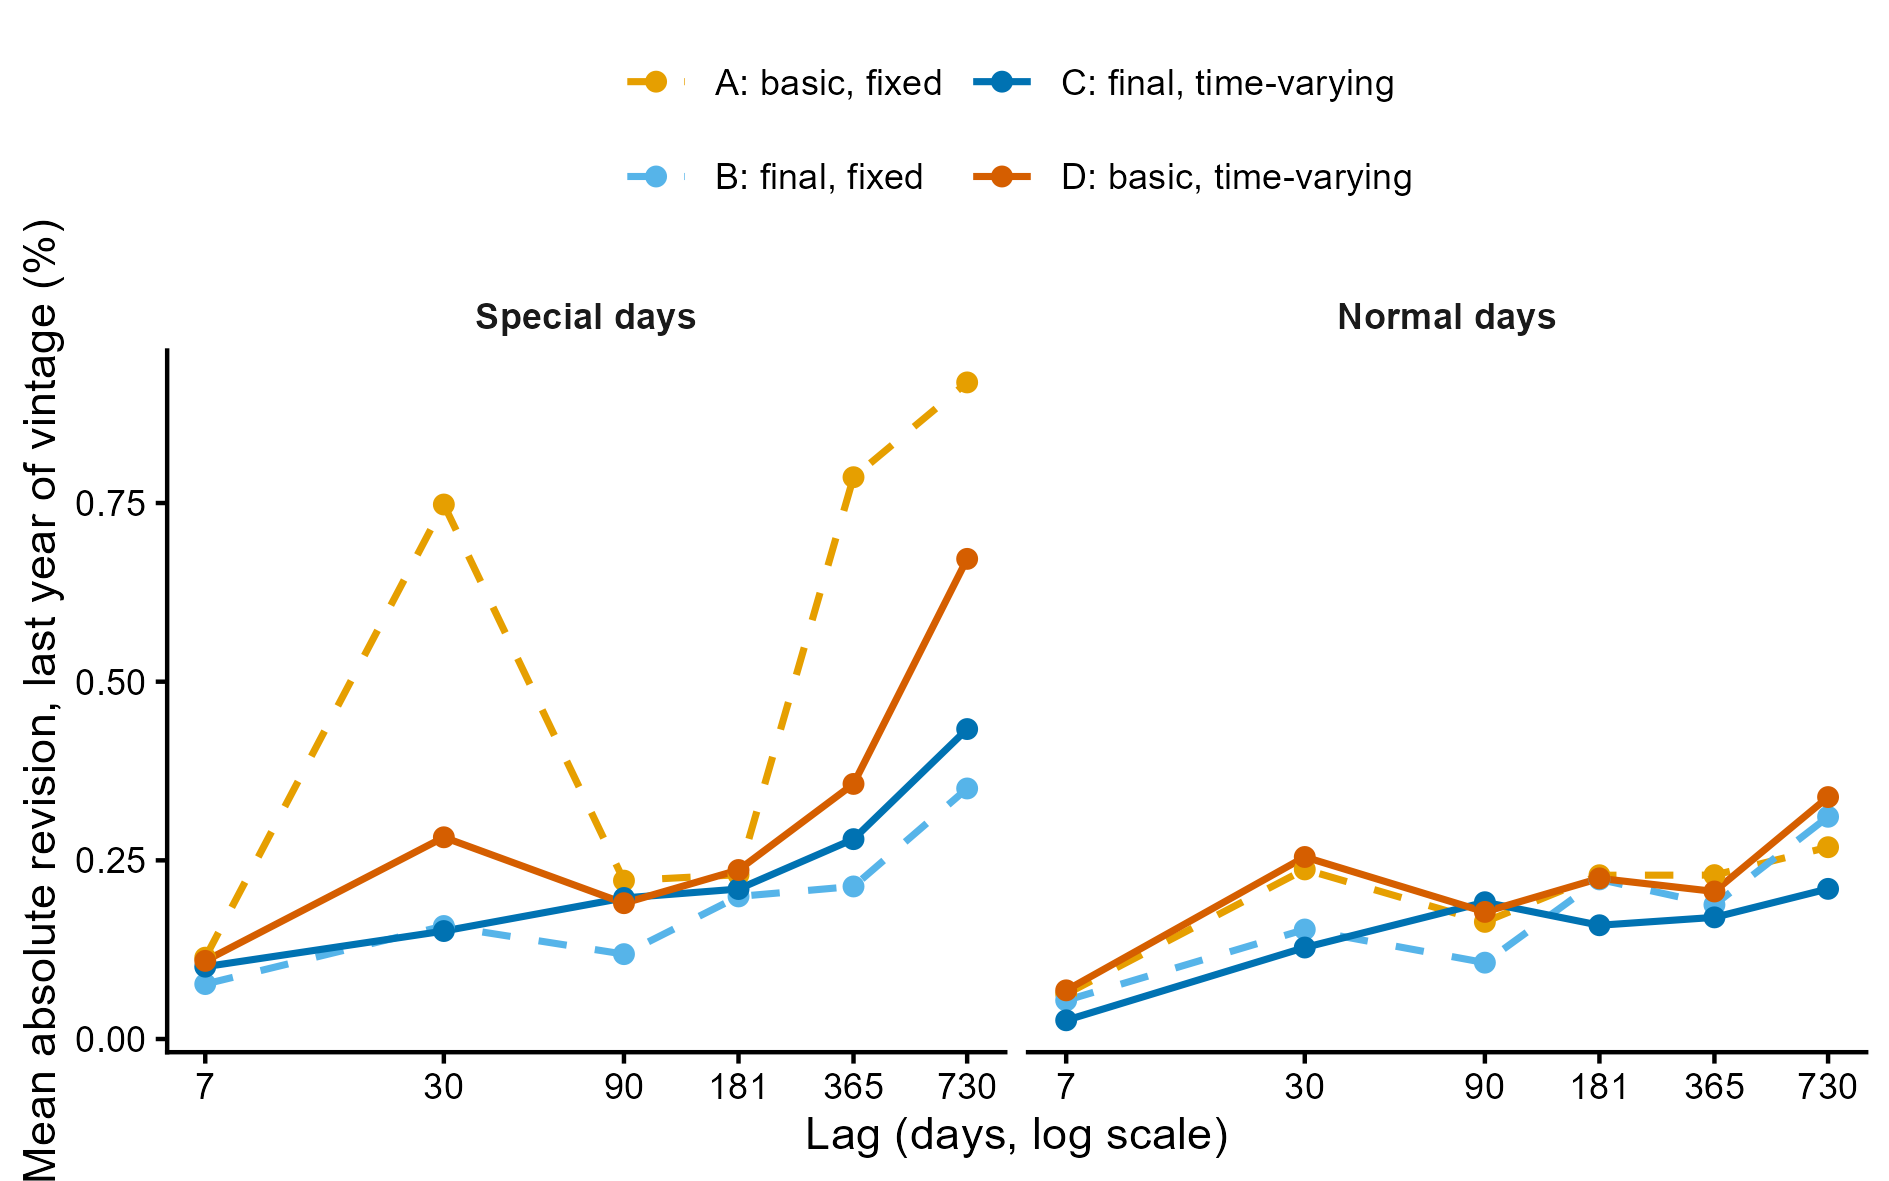
\includegraphics[width=0.85\textwidth]{figures/el_revisions_special_normal.png}
\caption{Electricity demand: revisions over the last year of each vintage, special days and other days, for the four specifications (RMAR, \%; lag on a log scale).}
\label{fig:rev_el}
\end{figure*}

The mechanism is the one already seen with the DMR. With the basic calendar and fixed coefficients (A), the full-sample model detects 28 outliers, 23 of which fall on holidays at weekends: as in e-invoicing, the outliers offset a holiday effect that should not apply on those days. Most of them are found in every vintage that covers their date, but not all: the Saturday All Saints' Day of 2025 is flagged in the vintage ending on 24 December 2025 but not in the one ending on 1 December; the Sunday New Year's Days of 2017 and 2023 are not flagged in the vintage ending on 1 January 2024 but are in the later ones; and the same episode around Epiphany 2024, a Saturday, is coded as a switch outlier on Friday 5 January in five estimates and as an additive outlier on 6 January in another. Each time such an outlier appears, disappears or changes, the adjusted value of those days is revised. With time-varying coefficients (D), no outlier falls on a special day: the coefficients absorb most of the specification error instead (Section~\ref{sec:el}), but they move as new data arrive, and the revisions of special days remain larger than with the final calendar. The basic calendar still leaves a trace in the outliers of D: a switch outlier on Sunday 30 October 2016 also involves the following Monday, the bridge before All Saints' Day on Tuesday 1 November, which the basic calendar does not model.

With the final calendar, the choice between fixed and time-varying coefficients is a trade-off. Time-varying coefficients give the smallest revisions on the historical sample and on the other days, and the smallest revisions overall at the end of the sample (0.15\% against 0.17\%). On special days, fixed coefficients do slightly better (0.19\% against 0.23\%): at the end of the sample the coefficients of the most recent holidays are filtered rather than smoothed estimates, and they are revised as new data arrive. The cost concerns a few days per year. Time-varying coefficients also give the most stable outlier configuration, and with it the most stable historical series. With fixed coefficients (B), the storm of 21 August 2015 and the three summer level shifts of 2023 are detected only in some vintages and not in the full sample, consistent with the largest single-day revision of B, about 65 thousand MWh, in exactly those vintages. With time-varying coefficients (C), the same outliers are found in all estimates, or in all but one, and the largest single-day revision on the historical sample is below 10 thousand MWh, against 32 thousand with D and 86 thousand with A.

\subsection{Electronic invoicing}
\label{subsec:rev_einv}

For e-invoicing only fixed coefficients are considered, since the estimated variance of time-varying coefficients was zero (Section~\ref{sec:einv}): we compare the basic calendar (A), with the twelve holidays on every day and three month-end dummies, and the final calendar (B), with 32 regressors. The days are split into three groups: holidays, on any day of the week (about 12 per year); month days, that is the last six days of the month, days 1, 15 and 20 and the last working Friday before a weekend month end (about 100 per year); and the other days.

\begin{table*}[t]
\centering
\caption{E-invoicing: revisions of the SCA series with the basic and final calendars (RMAR, \%, mean over six vintages) and outliers on holidays in the full-sample model.}
\label{tab:rev_einv}
\small
\begin{tabular}{@{}l l r r r r r r@{}}
\toprule
 & & Historical & \multicolumn{4}{c}{Last year of each vintage} & Outliers \\
\cmidrule(lr){4-7}
 & Calendar & sample & All days & Holidays & Month days & Other days & on holidays \\
\midrule
A & Basic (15 regressors) & 2.99 & 2.72 & 14.25 & 2.97 & 2.08 & 4 \\
B & Final (32 regressors) & 0.88 & 1.20 & 1.68  & 1.11 & 1.21 & 2 \\
\midrule
\multicolumn{2}{@{}l}{Change from A to B} & $-71\%$ & $-56\%$ & $-88\%$ & $-62\%$ & $-42\%$ & \\
\bottomrule
\end{tabular}
\begin{minipage}{\textwidth}
\footnotesize
\vspace{4pt}
Notes: multiplicative model, fixed coefficients. Basic calendar: twelve national holidays active on every day, last day of the month and the two days before; final calendar: Table~\ref{tab:einv}. Month days: last six days of the month, days 1, 15 and 20, last working Friday before a weekend month end. Holidays in B: the additive outlier on St.\ Stephen's Day 2020 (a Saturday) and the level shift at the end of the 2020 lockdown, on Republic Day.
\end{minipage}
\end{table*}

The gains are much larger than for electricity, because the calendar effects are much larger (Table~\ref{tab:rev_einv} and Figure~\ref{fig:rev_einv}). The final calendar reduces the revisions of the historical sample from 2.99\% to 0.88\%, and those of the last year of each vintage from 14.2\% to 1.7\% on holidays, from 3.0\% to 1.1\% on month days and from 2.1\% to 1.2\% on the other days. The improvement on the other days shows that a misspecified calendar does not only affect the days it models: the residual calendar effects enter the estimation of the seasonal components and of the outliers, and through them the whole series.

\begin{figure*}[t]
\centering
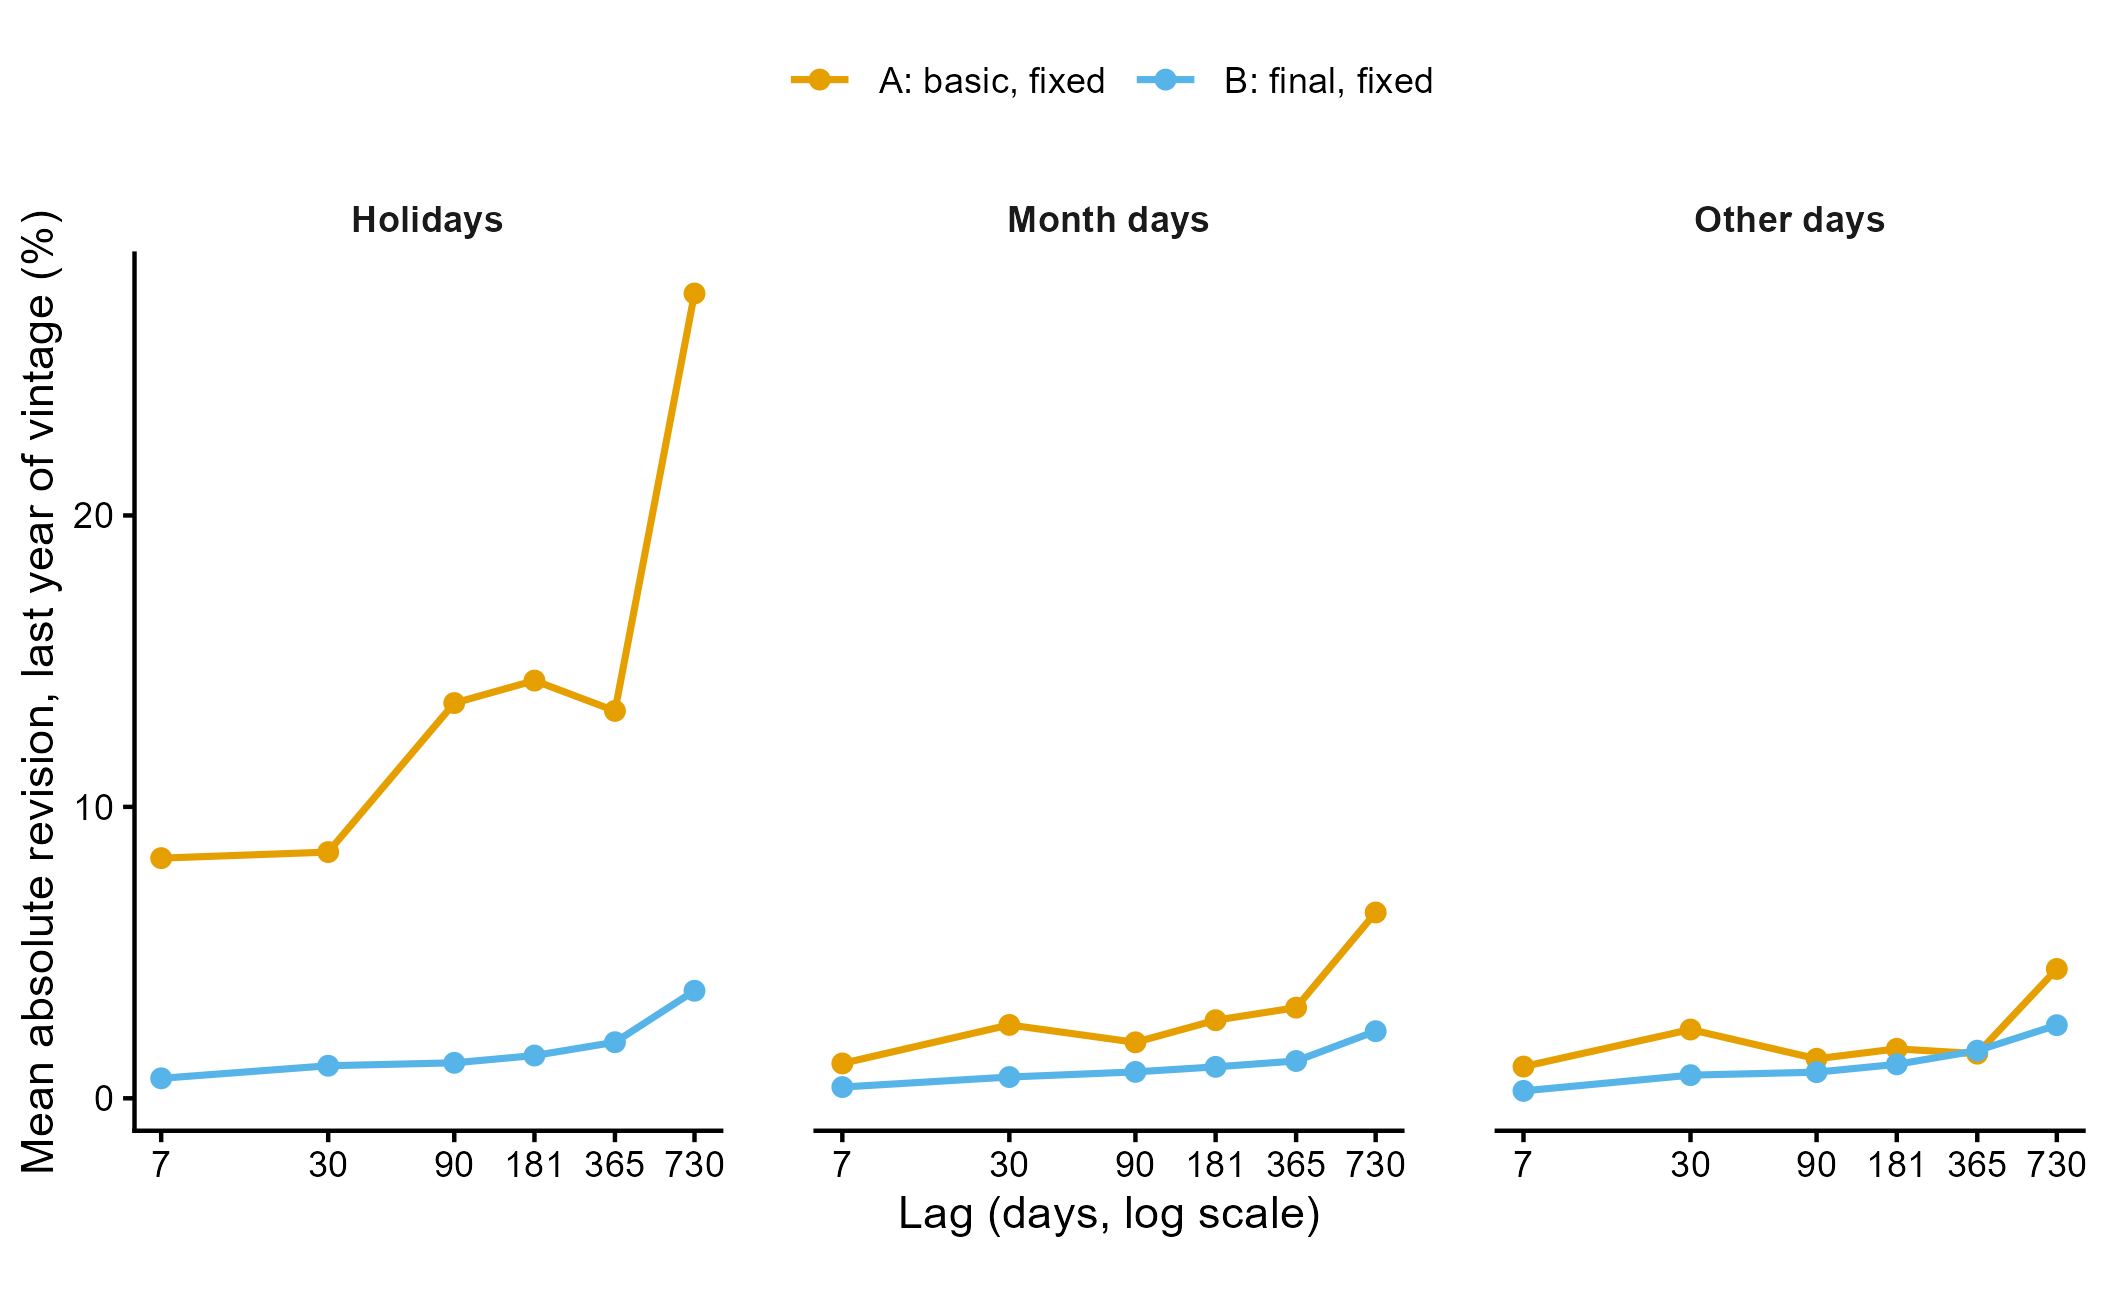
\includegraphics[width=0.95\textwidth]{figures/einv_revisions_by_group.png}
\caption{E-invoicing: revisions over the last year of each vintage, holidays, month days and other days, with the basic and the final calendar (RMAR, \%; lag on a log scale).}
\label{fig:rev_einv}
\end{figure*}

The outliers again show the mechanism. With the basic calendar, the outliers of the full-sample model fall mostly on holidays at weekends (All Saints' Day 2020, Assumption Day 2021, Christmas 2022 and New Year's Day 2023, all Sundays), plus a switch outlier on Sunday 30 April 2023, a month end. Only All Saints' Day 2020 is found in every estimate; the others come and go across vintages, and the same holiday may be coded as an additive outlier in one estimate and as a switch outlier in another (Christmas 2022). The largest single-day revisions of the historical sample, above 400\%, fall precisely on two of these days, New Year's Day 2023 and Assumption Day 2021. Moreover, the basic specification detects no level shift at all, not even the 2020 lockdown, which the final model estimates at $-34\%$: presumably, the residual calendar effects inflate the residual variance so much that genuine events no longer stand out. With the final calendar, the outliers of the full-sample model, which describe the pandemic and a few isolated events, are found in every estimate that covers their date (the start of the lockdown is dated three days later in the oldest vintage). The residual instability concerns Christmas at the weekend: Christmas 2021 (a Saturday) and 2022 (a Sunday) are not outliers in the full-sample model, but are flagged as additive outliers in the four intermediate vintages, which produces the largest single-day revision of B, about 100\%. A Christmas at the weekend is apparently not quite a normal weekend day; with only two cases in the sample, we leave it as an open point.

\subsection{Summary and caveats}

For both series, a calendar built with the DMR also gives more stable estimates, and the gains concentrate on the days the calendar is about: by 63\% (fixed coefficients) and 26\% (time-varying coefficients) on the special days of electricity, by 88\% on the holidays and 62\% on the month days of e-invoicing. Two caveats apply to both analyses. Each lag corresponds to a single vintage, and a single vintage can be unusual: even with C, four summer level shifts are not detected in the vintage ending on 2 October 2025, consistent with the higher revision of the historical sample at that lag. Hence the individual points in Figures~\ref{fig:rev_el} and~\ref{fig:rev_einv} are noisy and the averages are more reliable; and for electricity, revisions are small in absolute terms, below 1\% on average, so that the comparison is between specifications.

% =============================================================================
\section{What standard diagnostics see}
\label{sec:kde}

A common diagnostic for daily seasonal adjustment looks at the distribution of autocorrelations computed in rolling windows at the seasonal lags: residual seasonality shifts the distribution away from zero. We compute the autocorrelation at lags 7, 30 and 365, in rolling windows of four, three and two cycles (28, 90 and 730 days), on the first differences of the series (of the logs for e-invoicing), so that trends and level shifts do not inflate the autocorrelations, and compare the kernel density estimates for the raw series and the adjusted series with the basic and the final calendar (Figure~\ref{fig:kde}).

\begin{figure*}[t]
\centering
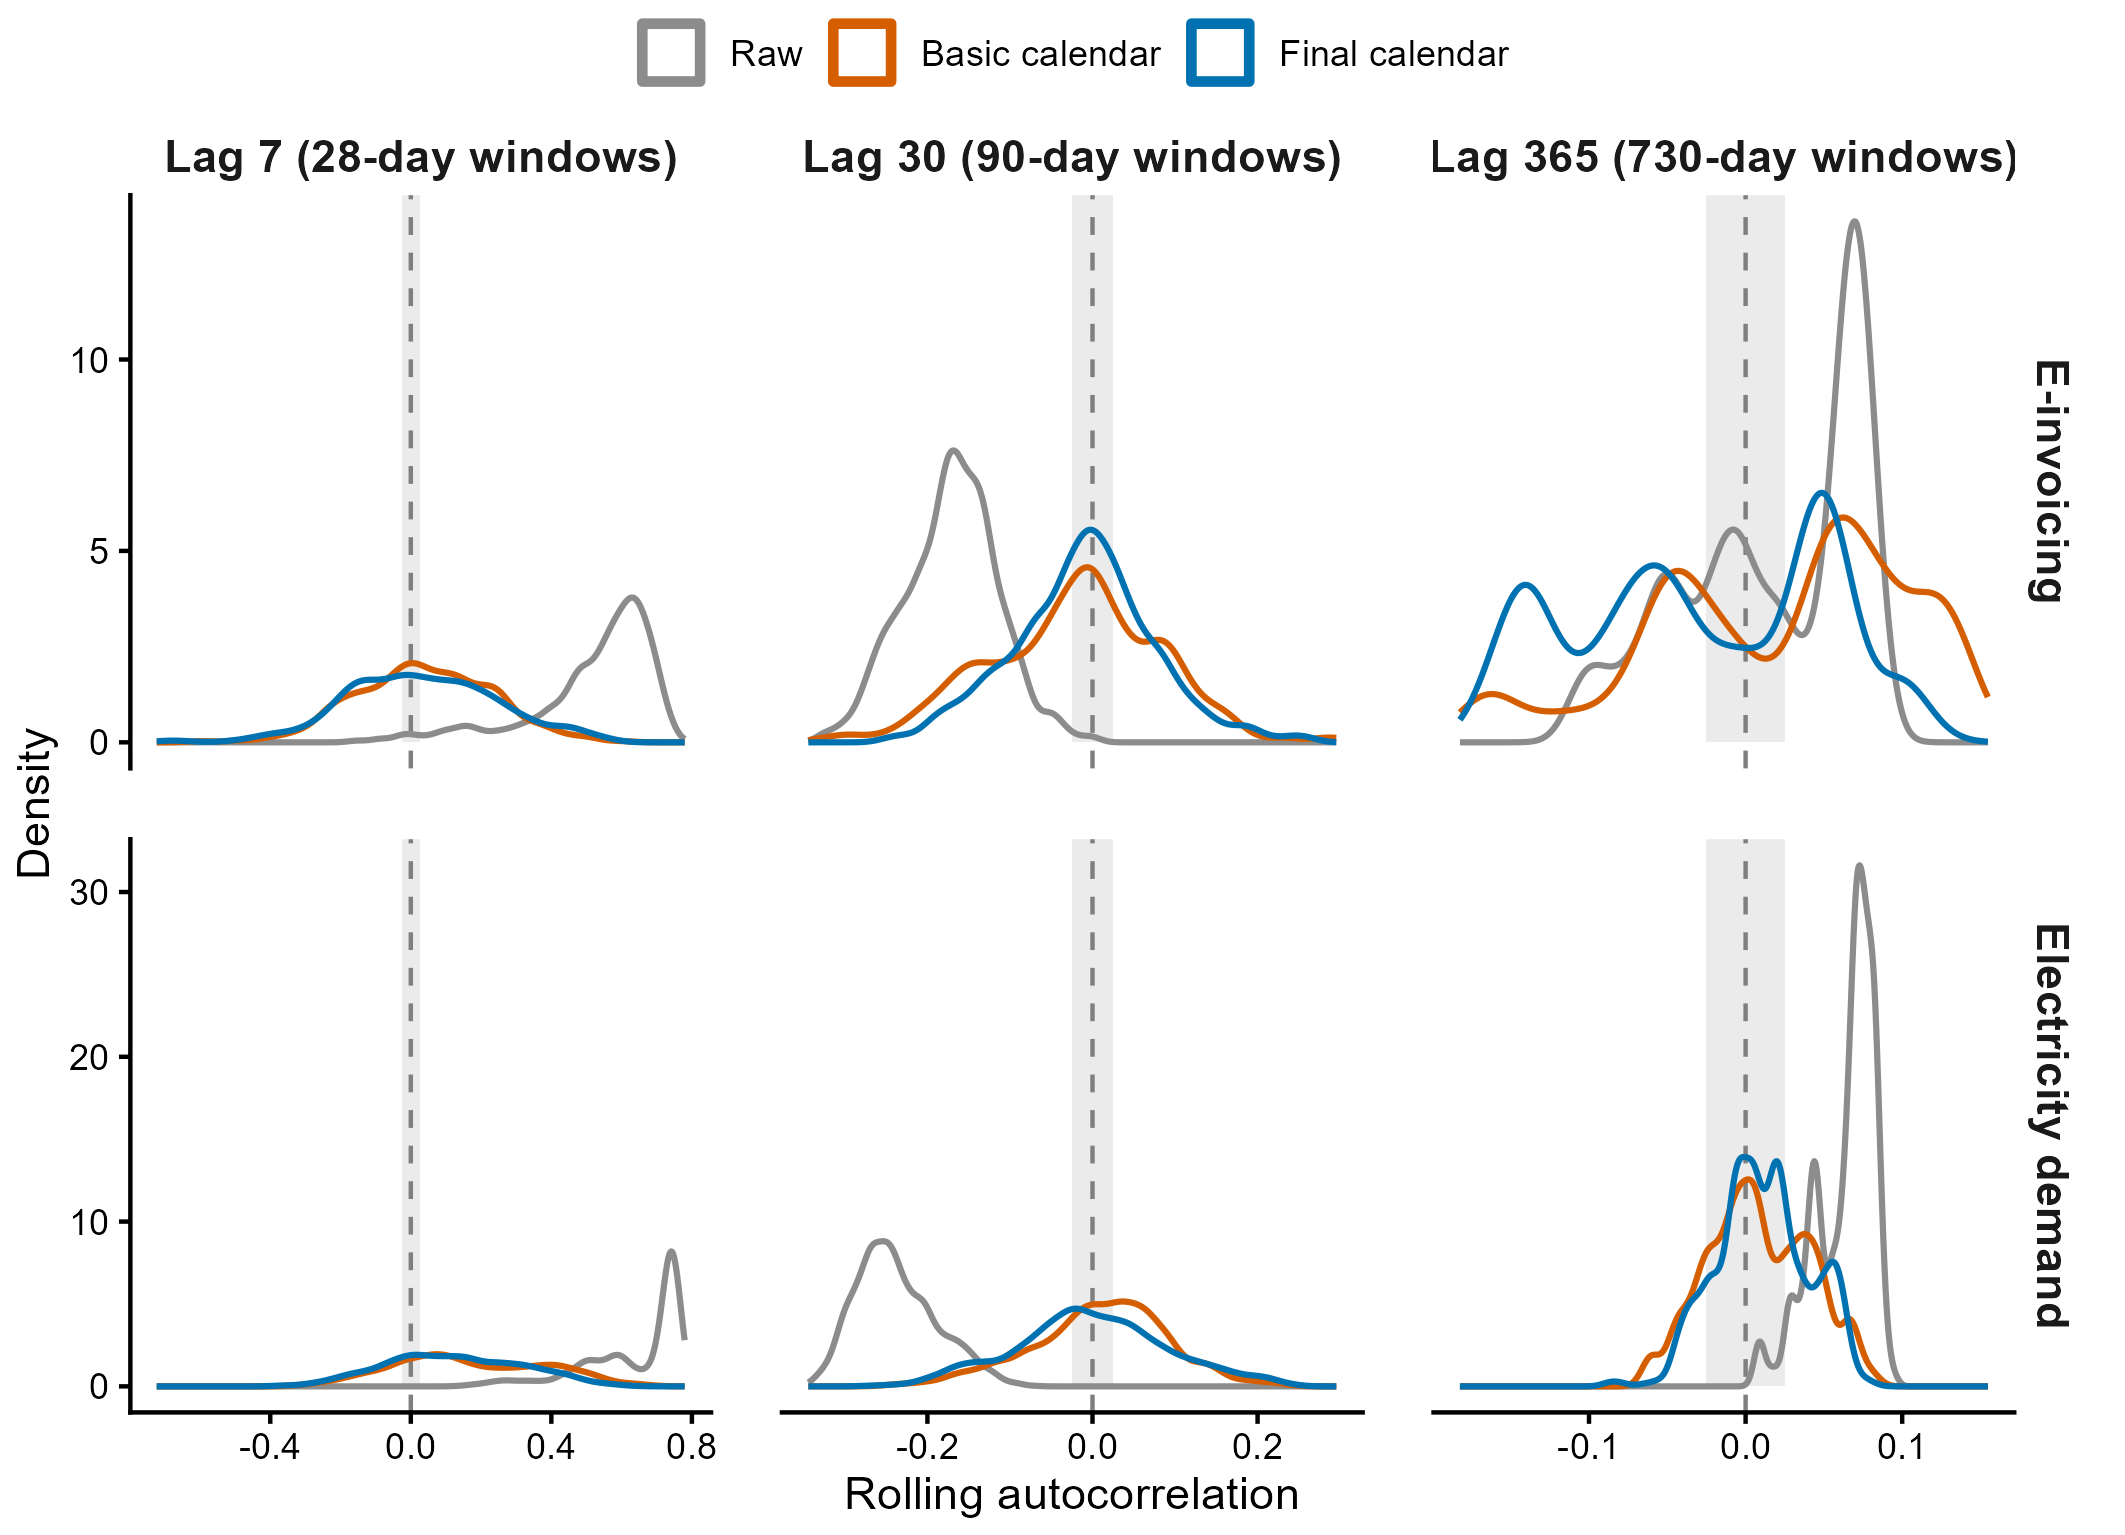
\includegraphics[width=\textwidth]{figures/kde_both.png}
\caption{Kernel densities of rolling autocorrelations at lags 7, 30 and 365, raw series and adjusted series with the basic and final calendars. Grey band: $\pm0.025$.}
\label{fig:kde}
\end{figure*}

The diagnostic clearly shows that seasonality has been removed: at lag 7 the raw series has rolling autocorrelations around 0.6--0.75, while the adjusted series are centred around zero; at lag 30 the raw series are shifted to negative values, partly because 30 days are four weeks and two days. However, the densities for the basic and the final calendar almost overlap, at every lag and for both series. The only visible difference is at lag 30 for e-invoicing, where the final calendar gives a slightly narrower density. At lag 365, with seven years of e-invoicing data, the 730-day windows overlap heavily and the multimodal densities reflect a few groups of consecutive windows rather than a distribution. \todo{report summary statistics of the rolling autocorrelations (median, deciles, mean absolute value) for the three versions}

The reason is structural: calendar effects concern a few days per year, which are diluted in windows that contain all days. The DMR, by grouping the days according to the mechanism of each effect, isolates exactly those days. Standard diagnostics of residual seasonality remain necessary, but they cannot be relied on to validate a daily calendar.

% =============================================================================
\section{Discussion}
\label{sec:discussion}

\subsection{Lessons for good practice}

Table~\ref{tab:compare} summarises the two calendars. Several lessons emerge.

\begin{table*}[t]
\centering
\caption{The two calendars at a glance.}
\label{tab:compare}
\small
\begin{tabular}{@{}p{3.2cm} p{5.4cm} p{5.4cm}@{}}
\toprule
 & E-invoicing & Electricity demand \\
\midrule
Calendar type       & Administrative: billing rules, fiscal deadlines & Production: plant activity, closures \\
Model               & Multiplicative (log), 2019--2025 & Additive (MWh), 2012--2025 \\
Intra-month effects & Strong: month end ($\times$8.6 on weekdays), days 1, 15 and 20, pre-month-end ramp & None \\
Around special days & Last working day before a weekend month end & Bridges, Easter window, Christmas period, mid-August \\
Weekends            & Sunday month end: 69 times a normal Sunday & Saturday holidays: a dedicated regressor \\
Effects over time   & Stable (estimated variance zero) & Gradual drift: holidays weaker by 10--18\% since 2012 \\
Calendar regressors & 32, fixed coefficients & 23, time-varying coefficients \\
\bottomrule
\end{tabular}
\end{table*}

\textit{The diagnostic transfers, the calendar does not.} The same building process leads to two very different calendars. Regressors must be built from the evidence of each series, not copied from another.

\textit{The effect of a special day depends on the day of the week.} A holiday, a month end or a deadline is relative to a normal day of the same type, and weekdays and weekends have very different base levels. One coefficient for all days is a compromise that over-corrects some days and under-corrects others; the signature is a median DMR below 1 on weekdays and above 1 at weekends, or the reverse. Holidays falling at weekends should, in most cases, be set to zero.

\textit{A fixed date is not necessarily seasonal.} When the effect of a fixed-date day depends on the day of the week, as for Christmas Eve in electricity demand, the annual seasonal component captures only its average across years.

\textit{Model the neighbours.} A drop over several days that is only partly modelled is absorbed by the local level and biases the effects of the modelled days.

\textit{The calendar is more than the official holidays.} Bridges, semi-closure days, month ends, deadlines and the last working day of the month have effects as large as some holidays.

\textit{Keep outliers and calendar effects apart.} An outlier on a holiday or on a nearby day signals a misspecified calendar, not an unusual event: in e-invoicing, before weekend holidays were set to zero, 11 of the 13 outliers fell on the weekend holidays themselves and offset the holiday coefficients. Outliers that absorb calendar effects hide the specification error and distort the adjusted series on exactly those days; moreover, they are not stable across vintages, and each time one appears or disappears the day is revised: with the basic e-invoicing calendar, by more than 400\% on two Sunday holidays (Section~\ref{sec:rev}). They can also mask genuine events: the same model detects no level shift during the 2020 lockdown. In a well-specified model, outliers describe events or data problems; in electricity demand, the summer level shifts and the storm of August 2015 point to weather effects that the calendar cannot capture.

\textit{Time variation must be tested on the complete calendar.} Free coefficients absorb specification errors and show variation that is not there; but removing the errors is not enough to rule time variation out. In e-invoicing the estimated variance was zero; in electricity a genuine drift remained. With the final calendar, time-varying coefficients have a small real-time cost on special days, whose most recent coefficients are revised as new data arrive, and a gain on all other days.

\subsection{Limitations}

\textit{Two-step estimation.} With time-varying coefficients, the calendar is estimated against a model with weekly seasonality only. Its local level absorbs part of multi-day drops, so that holidays remain slightly under-corrected: the median DMR of weekday holidays is 0.975--0.992 with the final calendar, below 1 for every weekday and in the Easter window. A joint estimation of time-varying calendar effects and annual seasonality would remove this bias, at a higher computational cost.

\textit{Weekly pattern within the year.} In August, the electricity DMR is above 1 at weekends (mostly 1.03--1.07) and below 1 on weekdays (mostly 0.94--0.98) over the whole month, with both calendars. This is not a calendar error: with plants closed, weekdays and weekends become closer, while the estimated weekly seasonality is the same throughout the year. The same effect explains the residual on 14 and 16 August.

\textit{Identification.} Separating a time-varying fixed-date effect from the annual seasonal component is difficult, and with few years of data the individual coefficient paths should be interpreted with caution; with a common variance, the coefficients of overlapping regressors, such as the midweek effect and the individual holidays, can offset each other.

\textit{The DMR.} The tolerance of $\pm5\%$ is a practical threshold, and the medians of small groups (eight Christmas Eves on working days) are uncertain. \todo{add bootstrap confidence intervals for the group medians, resampling months} The DMR has been applied here with one decomposition method; its behaviour with other methods for daily data \cite{ollech2021,proietti2023} remains to be checked.

\textit{Revisions.} The revision analysis uses one vintage per lag; more vintages, for instance one per month over 2024--2025, would make the comparison more robust.

% =============================================================================
\section{Conclusions}
\label{sec:conclusions}

Modelling the calendar well matters more for daily data than for monthly data, for four reasons. Special days are key days: month ends, holidays and bridges are the days users look at, and a wrong calendar distorts exactly them, by more than 20\% on some days of the month for e-invoicing with the basic calendar. Calendar effects are information in their own right: a month end worth almost nine weekdays of invoicing, or holiday effects on electricity that weaken by 10--18\% in fourteen years, tell something about the economy. At daily frequency, errors do not average out: a monthly total hides them, while a daily series shows each one as a false movement, or as an outlier that should have been a calendar effect. Finally, each series needs its own calendar.

The Day-to-Month Ratio, applied to groups of days chosen according to the mechanism of each effect, makes these errors visible on the adjusted series, where standard diagnostics barely see them, and a calendar built in this way also makes the most recent estimates more stable, above all on special days. Our recommendation is to build the calendar from the evidence of each series, one motivated regressor at a time, and to check it on the adjusted series, day by day.



\section*{Acknowledgements}
\todo{acknowledgements; data providers; co-authors, if any}

\bibliographystyle{SageV}
\bibliography{references}

\end{document}
